\documentclass[times, utf8, zavrsni]{fer}
\usepackage{booktabs}
\usepackage{pdfpages}
\usepackage{listings}
\usepackage{mathtools}
\usepackage{algorithmic}
\usepackage{algorithm}
\usepackage{amsmath}
\usepackage{relsize}

\renewcommand{\lstlistingname}{Isječak}
\DeclareMathOperator*{\argmax}{arg\,max}

\begin{document}

\lstset{
basicstyle=\linespread{1.2}\ttfamily\footnotesize,
keepspaces=true,
numbers=left,
frame=single,
showspaces=false,
numberstyle=\ttfamily,
columns=flexible,
extendedchars=true,
inputencoding=utf8,
literate={®}{{\textregistered}}1,
}

\thesisnumber{5709}

\title{Sustav za određivanje strukture teksta na temelju položaja pojedinih znakova}

\author{Herman Zvonimir Došilović}

\maketitle

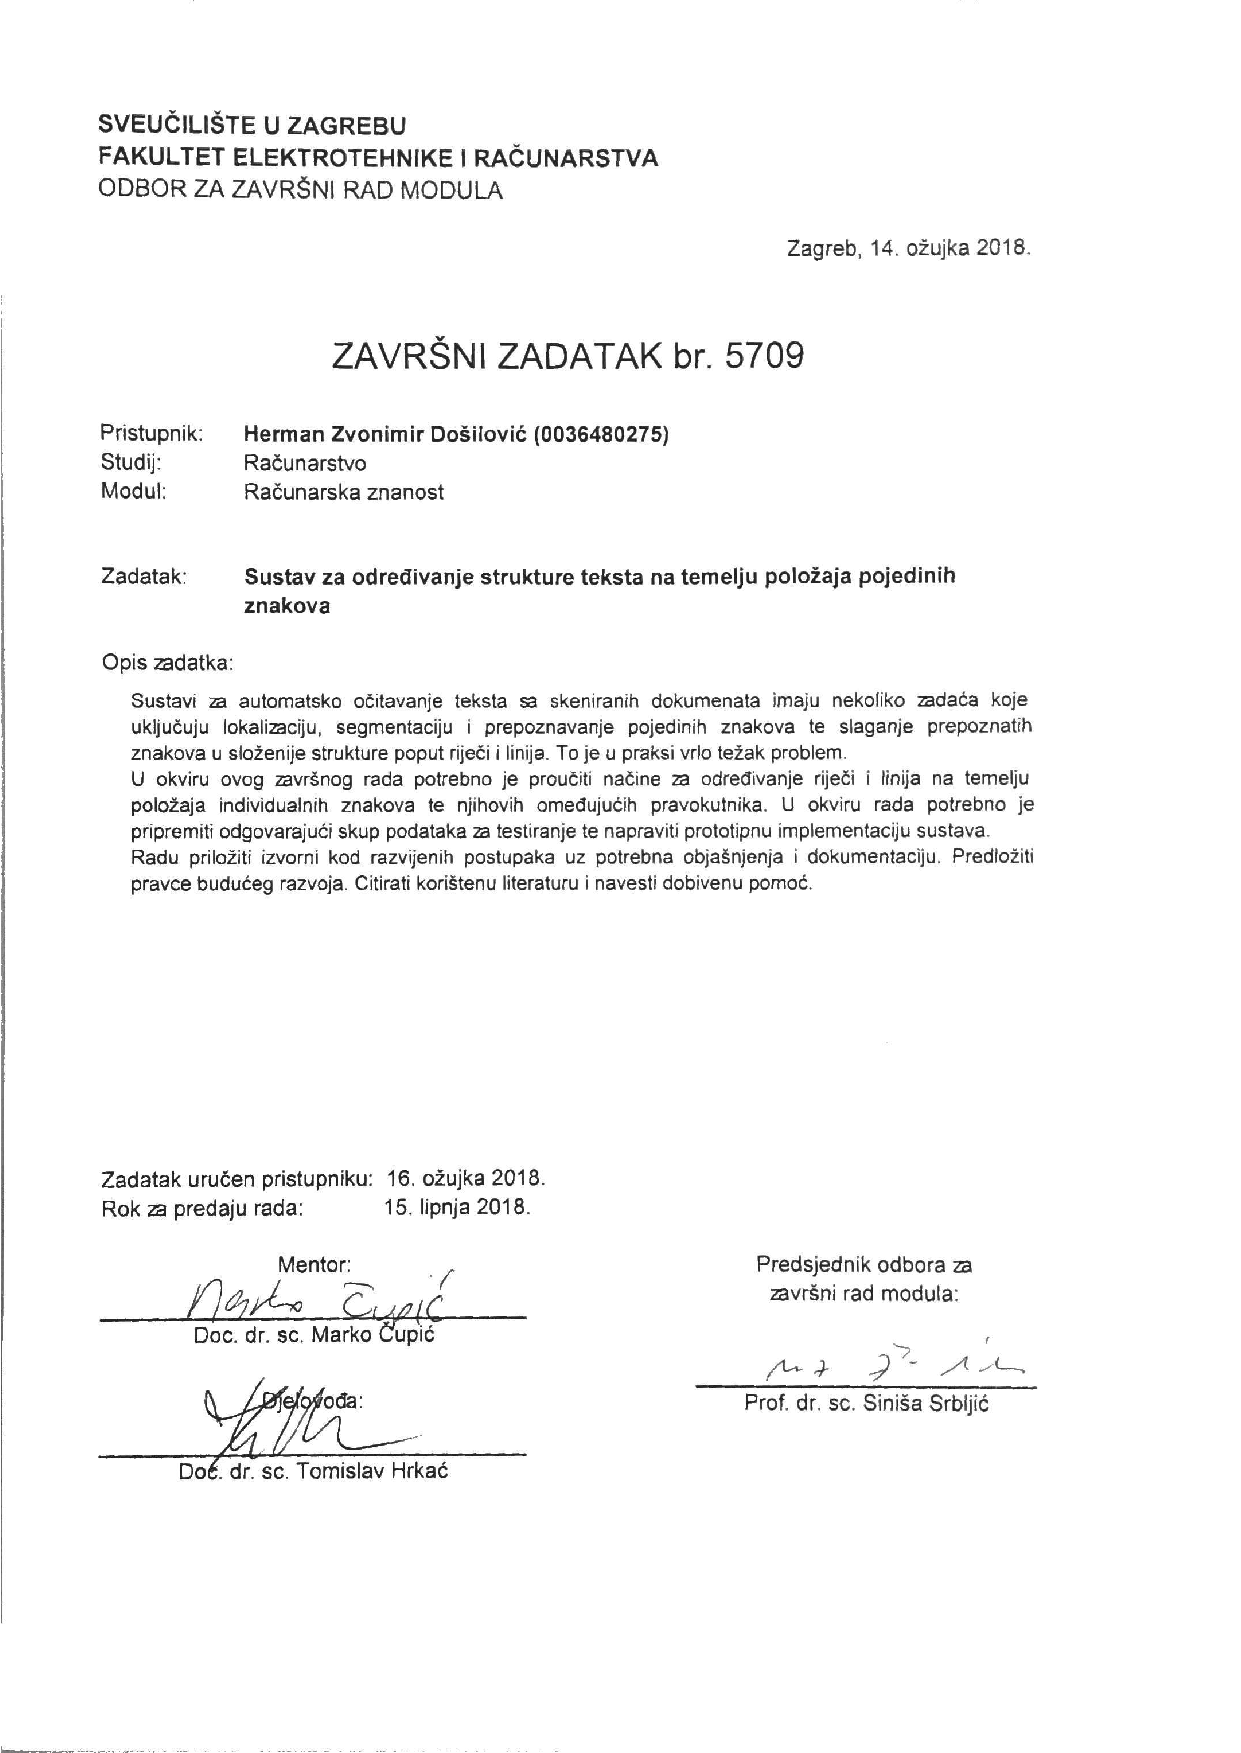
\includepdf[pages=-]{izvornik.pdf}

\zahvala{
    Zahvaljujem svom mentoru doc. dr. sc. Marku Čupiću na dozvoli za odabir vlastite teme i
    na strpljenju, poticaju i savjetima u razvoju rada.

    \

    Zahvaljujem tvrtki Microblink na danim sredstvima bez kojih ovaj rad ne bi bio moguć.
    Posebno zahvaljujem kolegama Jurici Cerovecu, Nenadu Mikši, Borisu Trubiću,
    Igoru Smolkoviču i Ivanu Jurinu koji su me svojim bogatim znanjem i iskustvom
    usmjeravali u razvoju rada.
}

\zahvala{
    Tko hoće da među vama bude najveći, neka vam bude poslužitelj! I tko hoće da
    među vama bude prvi, neka bude svima sluga. - Mk 10,43-44
}

\tableofcontents

\chapter{Uvod}
\chapter{Optičko raspoznavanje znakova}
Sustav za optičko raspoznavanje znakova \engl{optical character recognition} (u daljnjem tekstu: \emph{OCR-sustav})
pretvara sliku tiskanog teksta u digitalizirani format kojim možemo jednostavno manipulirati na računalu.
Iako je to ljudima jednostavan zadatak, računalima nije lako prepoznati tekst i pojedine znakove teksta sa slike
zbog velike raznolikosti jezika, fonta i stila kojim tekst može biti napisan.
Optičko raspoznavanje znakova je stoga vrlo zahtjevan problem i mnogo je istraživačkog truda uloženo u pokušaju
da se slike teksta pretvore u format koji računalo razumije. \citep{DBLP:journals/corr/abs-1710-05703}

\section{Primjene}

Osim tiskanog teksta, OCR-sustavi se koriste i u prepoznavanju znakova rukom pisanog teksta.
Prepoznavanje znakova rukom pisanog teksta je teži problem od prepoznavanja tiskanog teksta \citep{DBLP:journals/corr/abs-1710-05703} zato jer
se oblik znakova i njihov način pisanja razlikuje kod svake osobe (npr.\
rukopis odrasle osobe potpuno je drugačiji od rukopisa djeteta).
OCR-sustave za detekciju rukom pisanih znakova možemo podijeliti na dvije potkategorije:
\emph{on-line} i \emph{off-line}. \emph{On-line} OCR-sustavi detektiraju znakove dok
ih korisnici unose i to im omogućuje praćenje parametara poput: brzine pisanja, broja napravljenih poteza,
smjer pisanja, itd. \emph{Off-line} OCR-sustavi izvode se nad jednom slikom na kojoj se nalazi
sav sadržaj nad kojim je potrebno napraviti detekciju. Takvi sustavi nemaju dodatne informacije koje imaju
\emph{on-line} sustavi i zato je detekcija znakova kompliciranija \citep{DBLP:journals/corr/abs-1710-05703}. Slika \ref{fig:math-example-01} prikazuje primjer rezultata
\emph{off-line} OCR-sustava za detekciju rukom pisanih znakova.

\begin{figure}[htb]
    \centering
    \captionsetup{justification=centering,margin=2cm}
    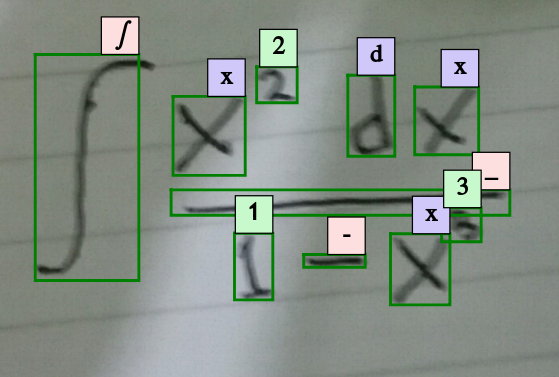
\includegraphics[height=4cm]{images/math-example-01.png}
    \caption{Rezultat \emph{off-line} OCR-sustava za detekciju znakova rukom pisanog teksta.}
    \label{fig:math-example-01}
\end{figure}

\pagebreak

OCR-sustavi imaju široku primjenu i možemo ih pronaći primjerice u detekciji
znakova na registarskim pločicama \citep{DBLP:journals/corr/Saghaei16a}, \citep{DBLP:journals/corr/abs-1802-09567},
u detekciji znakova sadržaja knjiga \citep{DBLP:journals/corr/abs-1802-10033},
\citep{Christy:2017:MDE:3172938.3075645} i
detekciji znakova na raznim dokumenatima \citep{DBLP:journals/corr/HarrajR15} \citep{verma2016ocr}. Na slici \ref{fig:receipt-example-01}
prikazan je primjer rezultata korištenja OCR-sustava za detekciju znakova na računima iz trgovine.
Slika \ref{fig:book-example-01} prikazuje rezultat OCR-sustava za detekciju znakova na tiskanim knjigama.

\begin{figure}[htb]
    \centering
    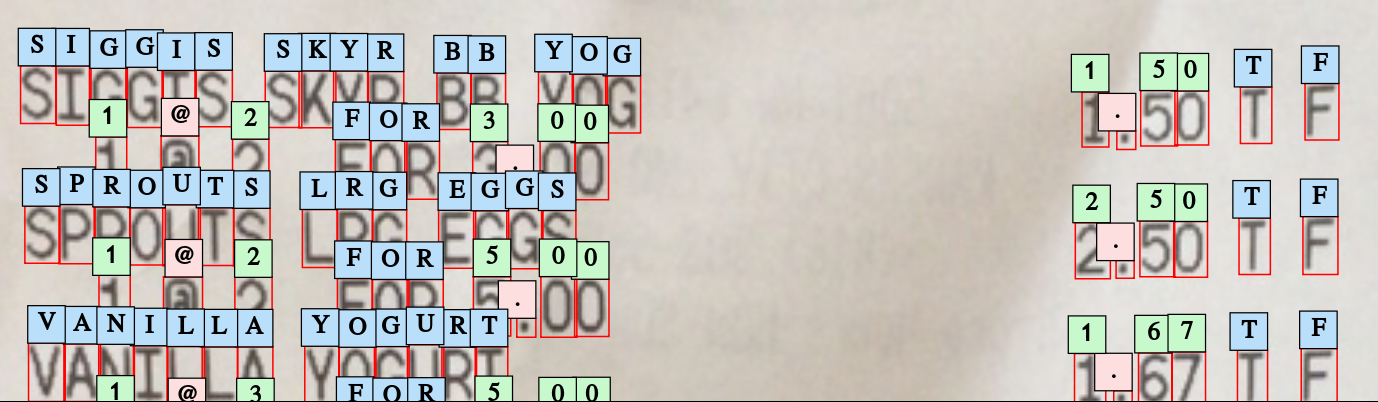
\includegraphics[width=\textwidth]{images/receipt-example-01.png}
    \caption{Rezultat OCR-sustava za detekciju znakova na računima iz trgovine.}
    \label{fig:receipt-example-01}
\end{figure}

\begin{figure}[htb]
    \centering
    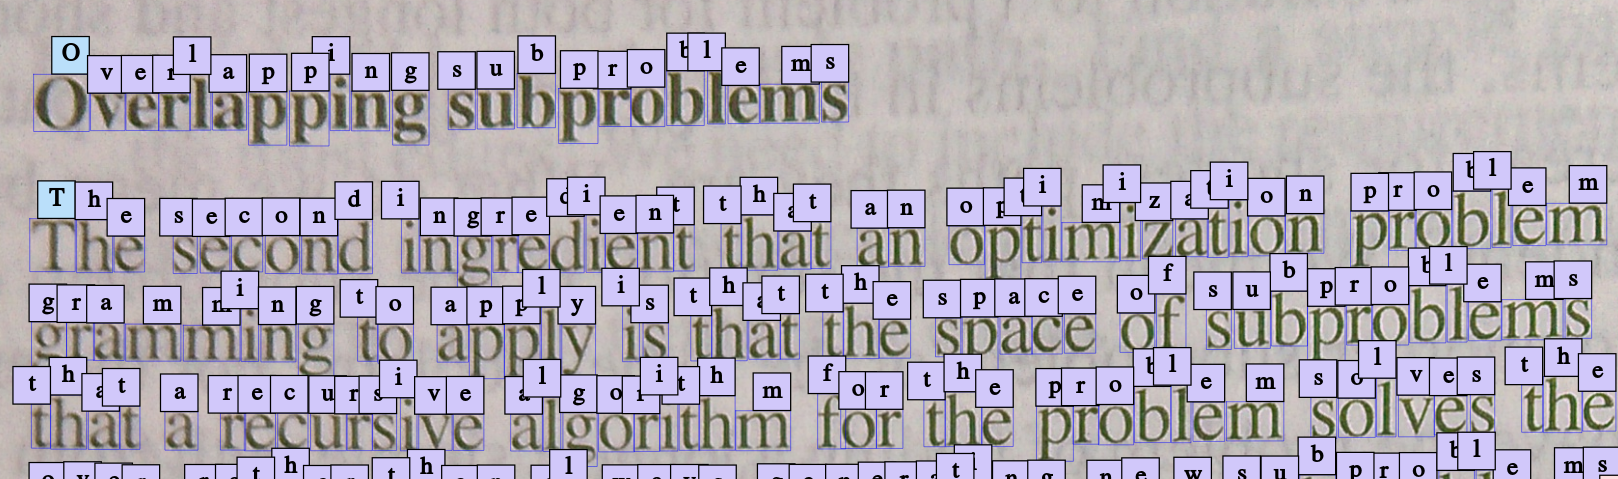
\includegraphics[width=\textwidth]{images/book-example-01.png}
    \caption{Rezultat OCR-sustava za detekciju znakova na tiskanim knjigama.}
    \label{fig:book-example-01}
\end{figure}

\pagebreak

\section{Komponente OCR-sustava}
\label{sec:komponente-ocr-sustava}
Optičko raspoznavanje znakova provodi se u nekoliko koraka \citep{DBLP:journals/corr/abs-1710-05703} \citep{kaur2016survey}:
\begin{enumerate}
    \item pribavljanje slike,
    \item predobrada,
    \item segmentacija znakova,
    \item izdvajanje značajki znakova,
    \item klasifikacija znakova i
    \item naknadna obrada.
\end{enumerate}

\subsubsection{Pribavljanje slike}

U prvom koraku OCR-a, pribavljanju slike, potrebno je pribaviti sliku nad kojom ćemo
provesti ostale korake. Sliku možemo pribaviti s raznih uređaja poput kamere fotoaparata,
mobilnog uređaja ili nekog drugog uređaja za digitalizaciju dokumenata \engl{scanner}.
Nakon prvog koraka, slika dokumenta nad kojim provodimo raspoznavanje znakova sastoji se
samo od slikovnih elemenata \engl{pixels} \citep{Vynckier:2018:HowOcrWorks}.
Slika \ref{fig:receipt-example-02} prikazuje primjer slike nad kojom možemo provesti
postupak raspoznavanja znakova. Primjetimo da slika može sadržati pozadinu koju bi
OCR-sustav trebao zanemariti.

\begin{figure}[htb]
    \centering
    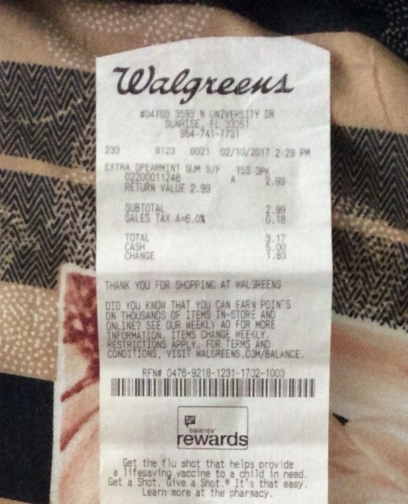
\includegraphics[height=7cm]{images/receipt-example-02.jpeg}
    \caption{Ulazna slika u OCR-sustav pribavljena kamerom mobilnog uređaja.}
    \label{fig:receipt-example-02}
\end{figure}

\subsubsection{Predobrada}

U predobradi slike OCR-sustavi često provode niz morfoloških transformacija i filtra nad pribavljenom slikom.
Cilj ovog koraka je povećati kvalitetu slike i smanjiti informacije na slici. Binarizacija je jedan od
potkoraka predobrade koji slike u boji ili u nijansama sive pretvara u crno-bijele. Osim binarizacije
koriste se neke morfološke transformacije poput dilatacije, rezanja i skaliranja.
Slika \ref{fig:binarization} prikazuje primjer slike prije i nakon binarizacije. \citep{Gulan:2016:Bacherlor},
\citep{DBLP:journals/corr/abs-1710-05703}, \citep{Jurin:2017:Master}

\begin{figure}[htb]
    \centering
    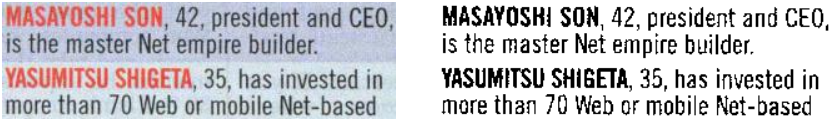
\includegraphics[width=\textwidth]{images/binarization.png}
    \caption{Prije binarizacije (lijevo) i nakon binarizacije (desno) \citep{Vynckier:2018:HowOcrWorks}.}
    \label{fig:binarization}
\end{figure}

\subsubsection{Segmentacija znakova}
\label{subsubsec:segmentacija}

Sljedeći korak, segmentacija znakova, je postupak segmentiranja slike u segmente unutar kojih se nalaze znakovi
koje želimo klasificirati. Jedan od pristupa segmentacije izvodi se s vrha prema dnu gdje se prvo
segmentiraju linije, zatim riječi i na kraju pojedini znakovi \citep{Jurin:2017:Master}, \citep{Vynckier:2018:HowOcrWorks}.
Prednost ovakvog pristupa je da uz lokaciju svakog znaka dobivamo i strukturu cijelog teksta, odnosno, znamo kojoj
liniji i kojoj riječi znak pripada. Nedostatak ovakvog pristupa je da ne postoje korekcijski mehanizmi kojima bismo
znak pridružili nekoj drugoj liniji ili riječi ako su prva dva koraka segmentacije linije ili riječi neispravni. \citep{Jurin:2017:Master}

Drugi pristupi poput \emph{ZICER OCR}\footnote{OCR-sustav tvrtke \emph{Microblink}, \url{https://microblink.com}} sustava izravno
izvode segmentaciju cijele slike na području koji predstavljaju znakove. Prednost takvog pristupa je da
možemo detektirati znakove teksta u kojemu nema riječi i linija, kao što je na primjer matematički izraz.
Nedostatak takvog pristupa je da gubimo informaciju o strukturi teksta i zato postoji potreba za razvojem dodatnog sustava koji bi znakove
grupirao u riječi, a riječi u linije \citep{Jurin:2017:Master}.
Slika \ref{fig:segmentation} prikazuje rezultat segmentacije pojedinih znakova.

\begin{figure}[htb]
    \centering
    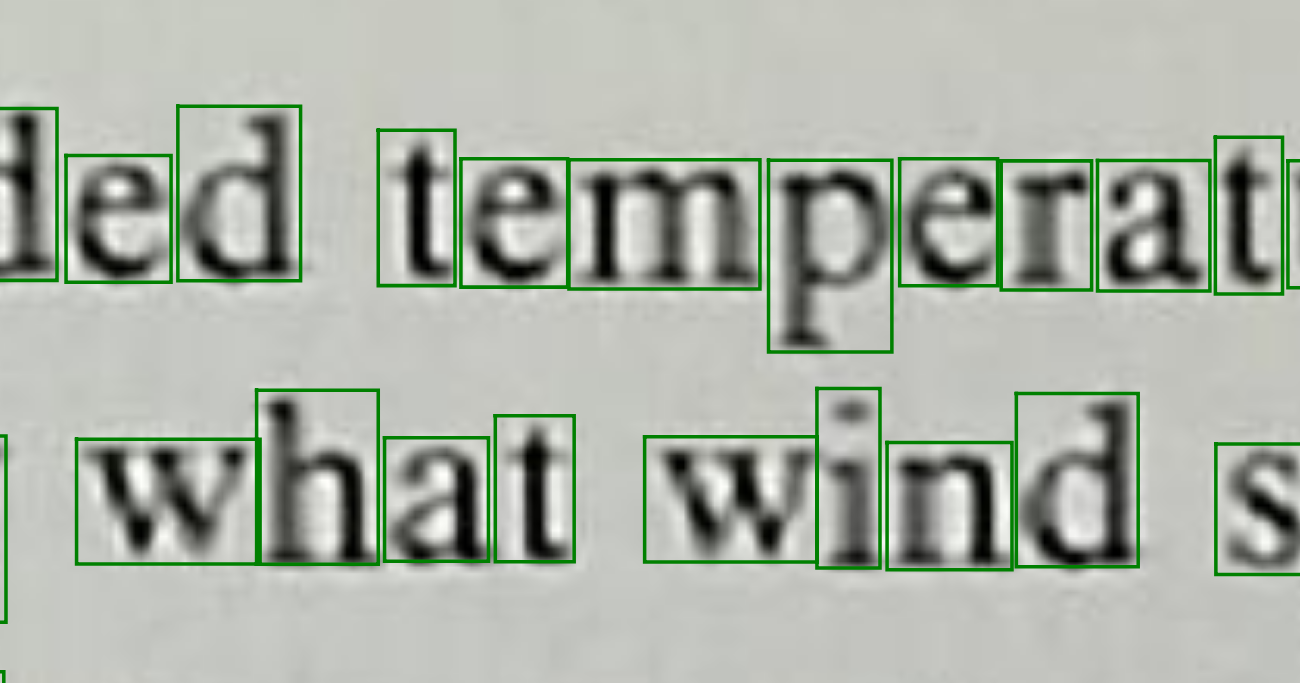
\includegraphics[height=4cm]{images/segmentation.png}
    \caption{Segmentacija znakova.}
    \label{fig:segmentation}
\end{figure}

\pagebreak

\subsubsection{Izdvajanje značajki}

Izdvajanje značajki pojedinog znaka podrazumijeva odabir značajki prema kojima će
se jedinstveno klasificirati svaki znak. Značajke poput geometrijskog oblika ili
statističkih svojstava mogu biti uzete u obzir prilikom klasifikacije. Važno područje istraživanja pripada
razmatranju koje i koliko značajki je potrebno uzeti u obzir za kvalitetnu i ispravnu
klasifikaciju. \citep{DBLP:journals/corr/abs-1710-05703}

\subsubsection{Klasifikacija}

Klasifikacija je najvažniji korak optičkog raspoznavanja znakova \citep{verma2012survey} \citep{zhu2016novel}
koji koristi izdvojene značajke za određivanje klase pojedinog znaka \citep{lehal1999feature} \citep{kaur2016survey}.
Statistički pristupi klasifikacije koriste diskriminativne funkcije za određivanje klase znaka \citep{DBLP:journals/corr/abs-1710-05703},
a u novije vrijeme koriste se duboke neuronske mreže \citep{Jurin:2017:Master}.
Neki od statističkih pristupa su: Bayesov klasifikator, klasifikator stablom odluke, umjetne neuronske mreže i
metoda k-najbližih susjeda \citep{DBLP:journals/corr/abs-1710-05703}.

2012. godine Krizhevsky i suradnici \citep{krizhevsky2012imagenet} objavili su rad koji je
označio prekretnicu u klasifikaciji i lokalizaciji objekata \citep{Jurin:2017:Master}. Slika
\ref{fig:deep-example-01} prikazuje arhitekturu \emph{AlexNet} koja je pobijedila na natječaju
\emph{ImageNet 2012} u području klasifikacije objekata. \citep{Jurin:2017:Master}

\begin{figure}[htb]
    \centering
    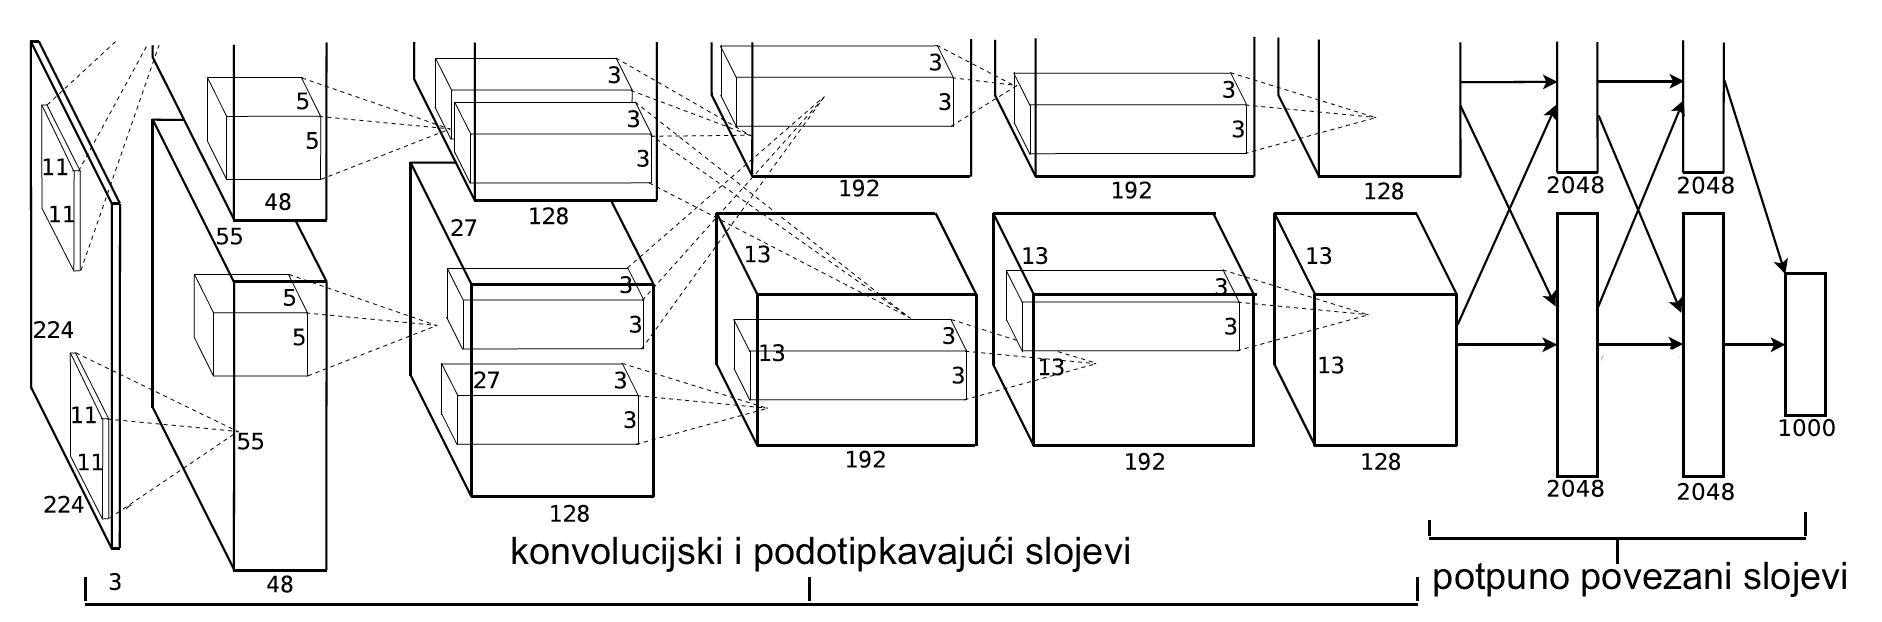
\includegraphics[width=\textwidth]{images/deep-example-01.png}
    \caption{Arhitektura \emph{AlexNet} \citep{Jurin:2017:Master}}
    \label{fig:deep-example-01}
\end{figure}

\subsubsection{Naknadna obrada}

Nakon klasifikacije znakova slijedi njihova naknadna obrada koja se koristi kako
bi se poboljšali OCR-rezultati. Jedan od pristupa postprocesiranja koristi rezultate
više različitih klasifikatora koji mogu biti korišteni slijedno, paralelno ili hijerarhijski.
Nakon toga rezultati klasifikatora se kombiniraju različitim pristupima. \citep{DBLP:journals/corr/abs-1710-05703}
Kao što je spomenuto u \ref{subsubsec:segmentacija} segmentacija koja se ne provodi s vrha prema
dnu nema informaciju o strukturi teksta i zato je potrebno razviti dodatan
\textbf{sustav za određivanje strukture teksta na temelju položaja pojedinih znakova}.

Schulz i suradnici \citep{schulz2017multi} 2017. godine predstavili su arhitekturu
tzv. \emph{post-correction} OCR-sustava kojim su pokazati na koji način su
adaptirali generički sustav za naknadnu OCR-rezultata koristeći domensko znanje
za konkretan problem koji su rješavali. Ovim pristupom ostvarili su bolje rezultate
za konkretni problem nego što su ostvarili koristeći postojeći generički sustav za
naknadnu obradu OCR-rezultata.

\

\begin{figure}[htb]
    \centering
    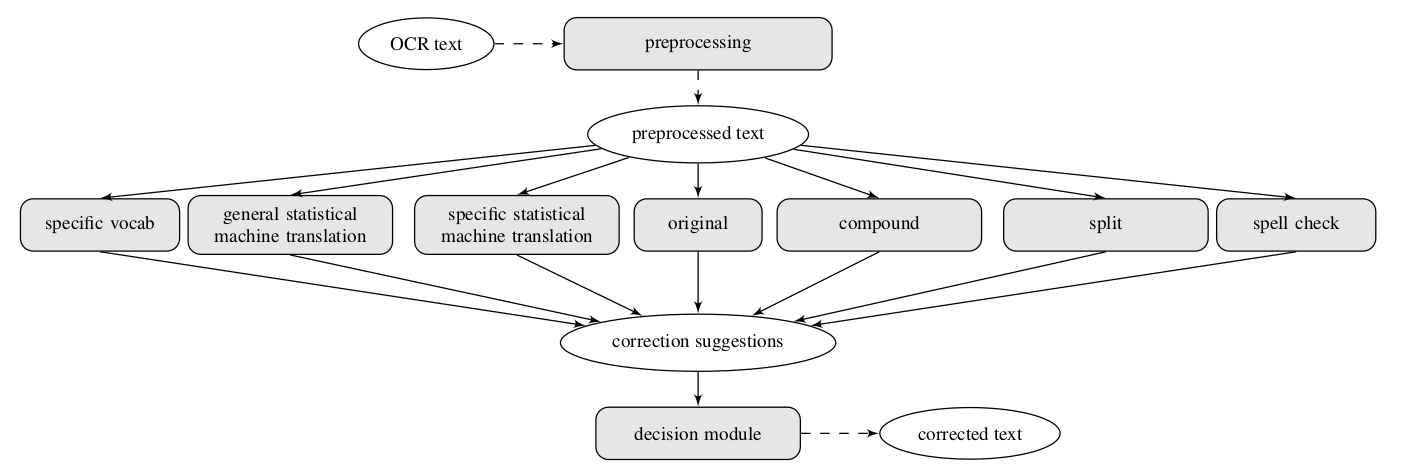
\includegraphics[width=\textwidth]{images/post-correction-example-01.png}
    \caption{Arhitektura \emph{post-correction} OCR sustava \citep{schulz2017multi}}
    \label{fig:post-correction-example-01}
\end{figure}

\chapter{Određivanje strukture teksta}

\begin{figure}[htb]
    \centering
    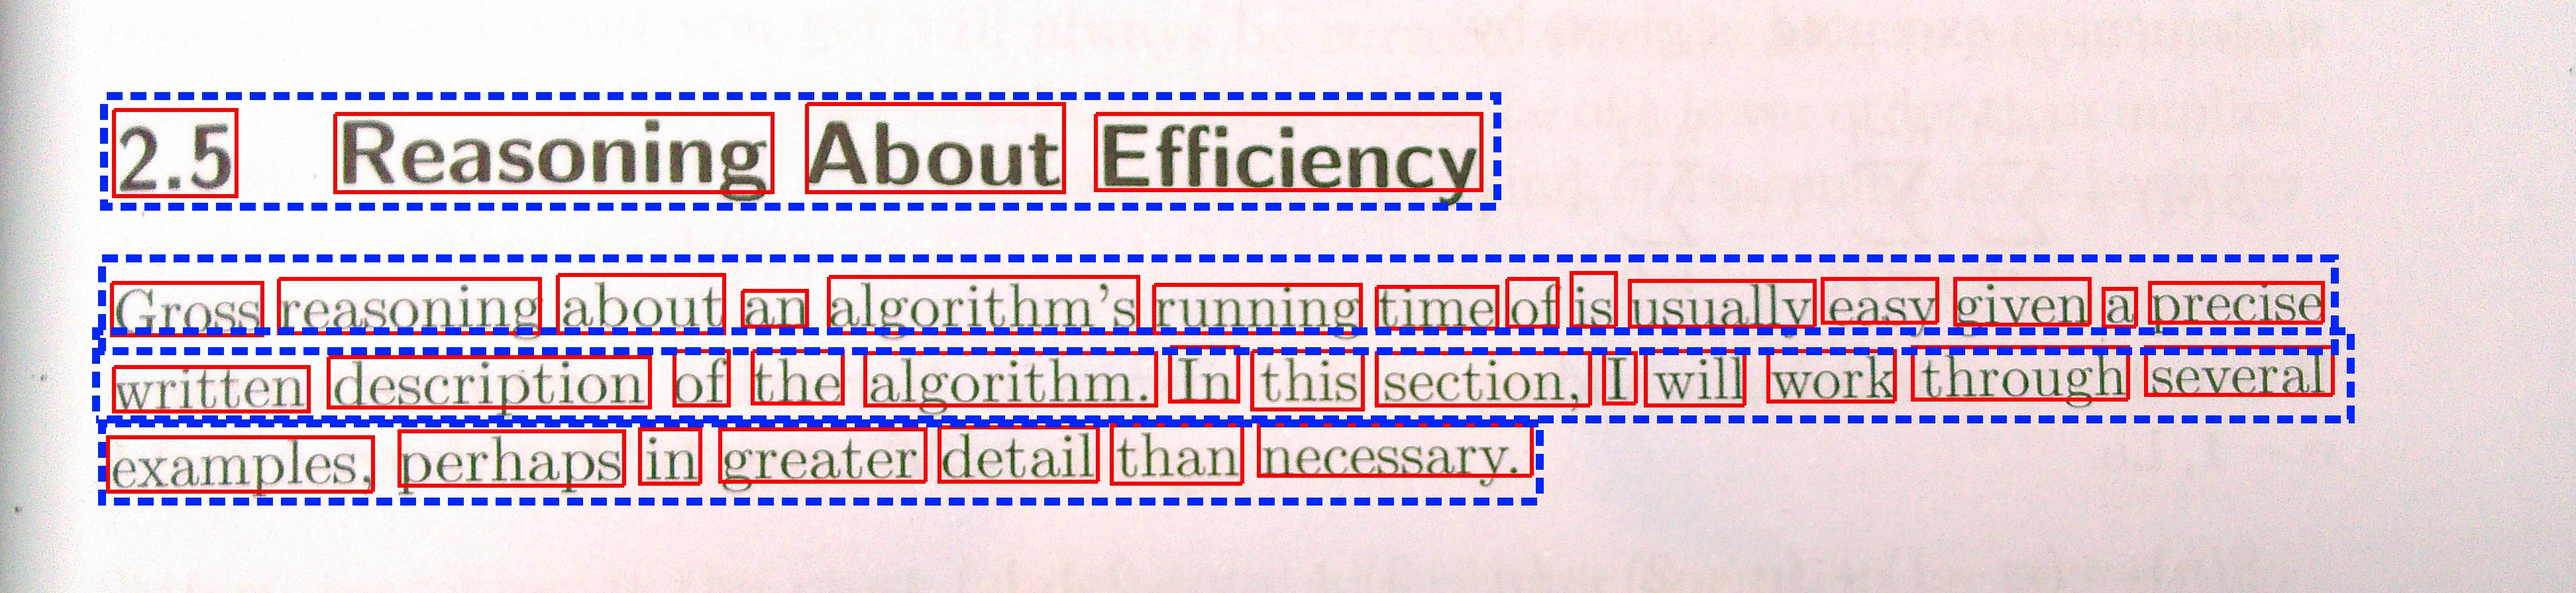
\includegraphics[width=\textwidth]{images/text-segmentation-01.jpg}
    \caption{Segmentacija linija (plavo) i riječi (crveno) unutar linije.}
    \label{fig:text-segmentation-01}
\end{figure}

Sustavi za određivanje strukture teksta na temelju OCR-rezultata sastavni su dio OCR-sustava. Određivanje strukture teksta
podrazumjeva segmentaciju linija i segmentaciju riječi unutar linije. Neke tehnike segmentacije
znakova i njihove klasifikacije nemaju informaciju o tome kojoj liniji i riječi pojedini znak pripada.
Prednost takvog pristupa je da takav OCR-sustav možemo koristiti nad slikama koje ne sadrže linije,
kao što su na primjer slike matematičkih izraza \citep{Jurin:2017:Master}. Nedostatak je što nakon klasifikacije
moramo razviti sustav koji će znakove naknadno obraditi da bismo odredili strukturu teksta \citep{Jurin:2017:Master}.

Tekst na slici može biti podijeljen na linije ili blokove, a u bloku
tekst možemo podijeliti na linije. Unutar jedne linije znakove možemo grupirati riječi. Način na
koji će se odrediti struktura teksta uvelike ovisi o problemu koji riješavamo i kakve rezultate
želimo dobiti. Tekst na slici \ref{fig:text-segmentation-01} podijeljen je na linije (plavo), a unutar
svake linije na riječi (crveno).

Tain i suradnici \citep{DBLP:journals/corr/TianPHLYT16} predlažu sustav za određivanje strukture teksta
koji će osim određivanja kojoj liniji pojedini znak pripada znati izbaciti tzv. \emph{false positive}
znakove odnosno znakove koje je OCR-sustav prepoznao, a zapravo u tekstu ne postoje. Njihov sustav temelji
se na \emph{min-cost flow network} modelu koji objedinjuje izbacivanje \emph{false positive} znakova i
pronalazak strukture teksta. Na temelju međusobne pozicije između dva prepoznata znaka i
dodatnog parametra kojeg dobivaju od klasifikatora, a koji označava vjerojatnost ispravne detekcije, grade težinski
usmjereni graf (Slika \ref{fig:text-flow}) kojim svoj problem modeliraju \emph{min-cost flow network} modelom.

\begin{figure}[htb]
    \centering
    \captionsetup{justification=centering,margin=2cm}
    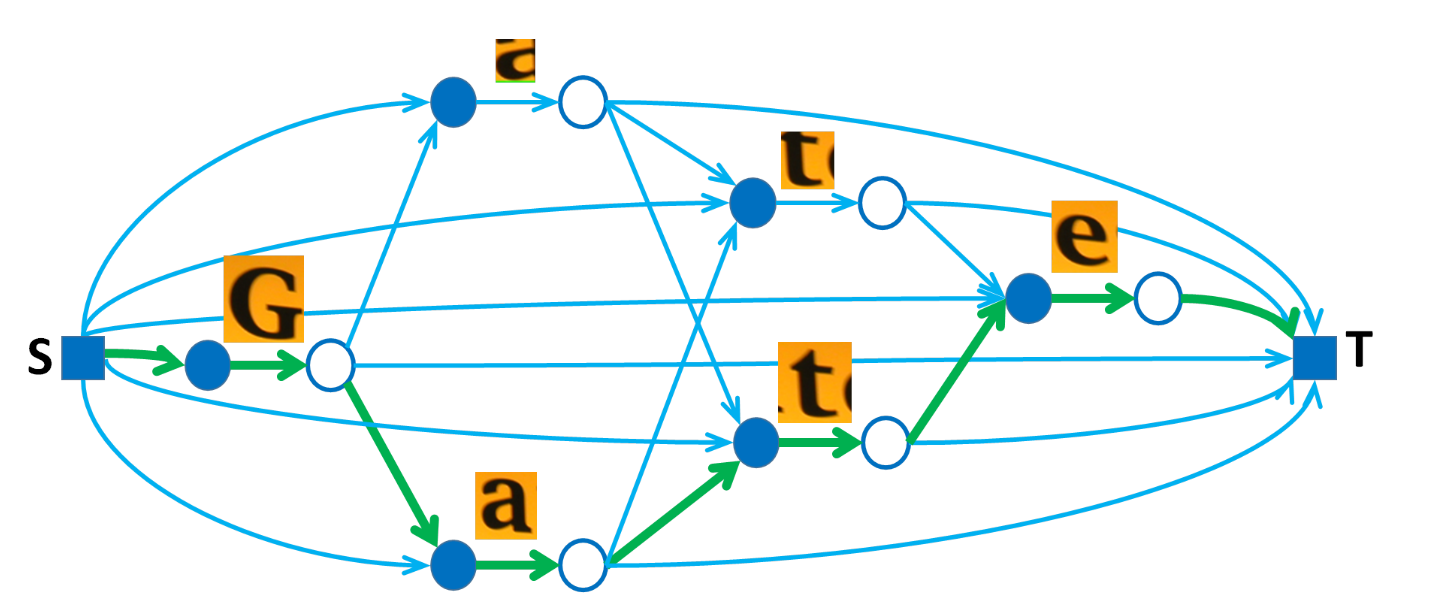
\includegraphics[height=6cm]{images/text-flow.png}
    \caption{Težinski usmjereni graf temeljen na \emph{min-cost flow network} modelu \citep{DBLP:journals/corr/TianPHLYT16}.}
    \label{fig:text-flow}
\end{figure}

\pagebreak

Zhu i suradnici \citep{zhu2016novel} predložili su novu arhitekturu (slika \ref{fig:novel-ocr}) OCR-sustava koji se temelji na empirijskim
rezultatima koji su pokazali da sadržaj riječi ne ovisi samo o dijelu teksta u kojem se ta riječ
nalazi nego i o susjednim dijelovima teksta. Njihov novi OCR-sustav radi dvostruku analizu strukture
teksta -- prije klasifikacije i nakon klasifikacije. Prva analiza strukture teksta omogućuje im da odrede
strukturu teksta u blokovima, a druga analiza strukture teksta im omogućuje da poprave pogreške u klasifikaciji.
Njihova nova arhitektura predstavlja hibridni OCR-sustav koji iskorištava rezultate analize strukture teksta.

\

\begin{figure}[htb]
    \centering
    \captionsetup{justification=centering,margin=2cm}
    \fbox{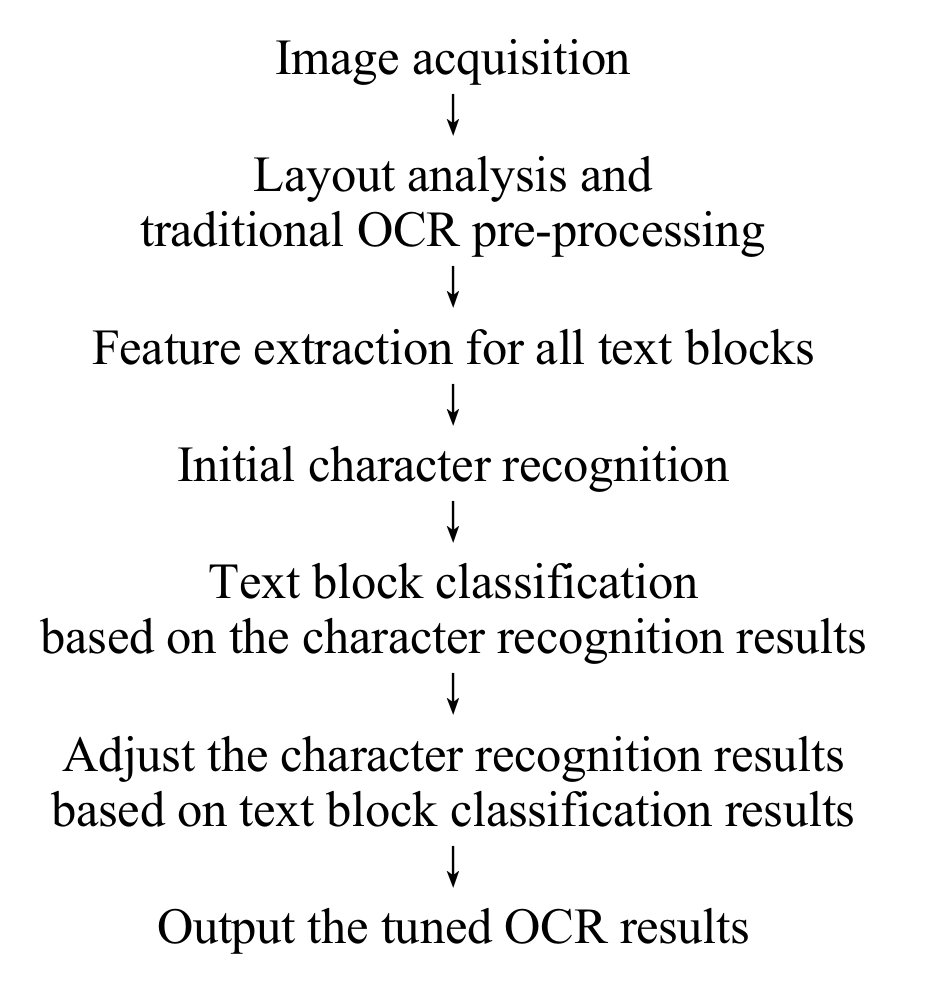
\includegraphics[height=7cm]{images/novel-ocr.png}}
    \caption{Arhitektura novog OCR-sustava kojeg predlažu Zhu i suradnici \citep{zhu2016novel}.}
    \label{fig:novel-ocr}
\end{figure}

\pagebreak

Yin i suradnici \citep{yin2007handwritten} pronalaze linije u tekstu povezujući znakove u težinski
graf nad kojim provode Kruskalov algoritam za pronalazak minimalnog razapinjujućeg stabla. Njihov
pristup ne koristi rezultate klasifikacije, nego koriste povezane komponente koje im predstavljaju
znakove i koje pronalaze koristeći algoritam temeljen na praćenju kontura \engl{contour tracing}.
Slika \ref{fig:mst-example-01} prikazuje rezultat pronalaska linija teksta u rukom pisanom dokumentu na
Engleskom jeziku.

\

\begin{figure}[htb]
    \centering
    \captionsetup{justification=centering,margin=2cm}
    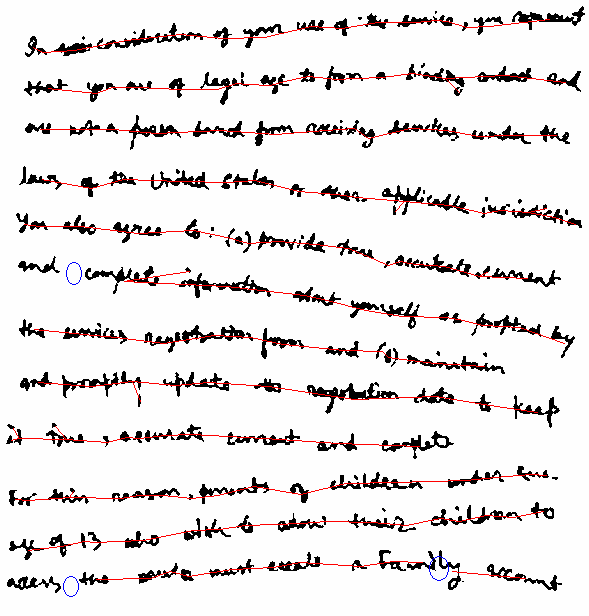
\includegraphics[height=8cm]{images/mst-example-01.png}
    \caption{Rezultat pronalaska linija teksta u rukom pisanom dokumentu na Engleskom jeziku \citep{yin2007handwritten}}
    \label{fig:mst-example-01}
\end{figure}

Motivirani njihovim radom Pan i suradnici \citep{pan2011hybrid} predstavili su sličan pristup
koji u težinama grafa uzima u obzir dodatne težine koje su učene MCE \engl{minimum classification error} mjerom.

Još jedan pristup predložili su Yin i suradnici \citep{DBLP:journals/corr/abs-1301-2628} koji koriste
tehniku hijerahijskog grupiranja koji postupno spaja linije koje dijele znakove dok god
postoje linije koje se mogu spojiti. \citep{DBLP:journals/corr/TianPHLYT16}

Liang i suradnici \citep{liang1996document} predlažu heuristički algoritam za određivanje sturkture
teksta. Algoritam radi horizontalnu projekciju (slika \ref{fig:histogram-projection}) omeđujućih pravokutnika na jednu ravninu i pronalazi
vrhove i doline u histogramu koji prikazuje frekvencije pojavljivanja projektiranih pravokutnika.
Osim ovog pristupa predložili su još jedan koji spaja dva znaka u jednu cjelinu ako i samo ako
su dva znaka dovoljno blizu da ih ima smisla spojiti. Gupta i suradnici \citep{gupta2006document} također koriste razne heuristike prema kojima
povezuju susjedne omeđujuće pravokutnike.

\pagebreak

\begin{figure}[htb]
    \centering
    \captionsetup{justification=centering,margin=2cm}
    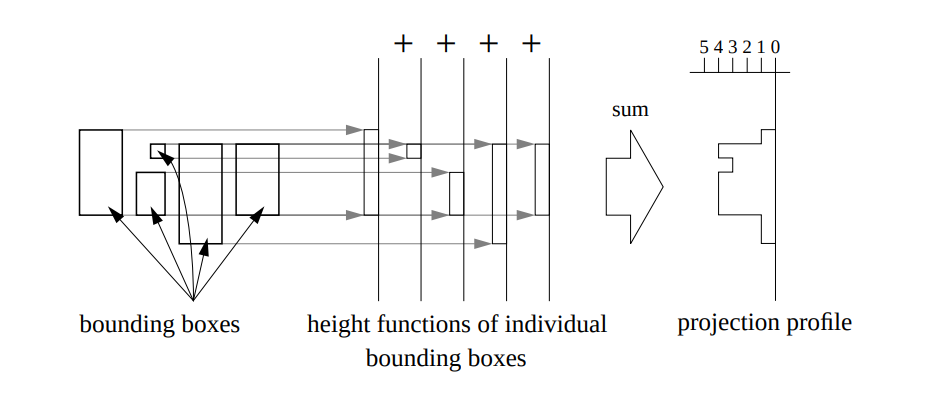
\includegraphics[height=6cm]{images/histogram-projection.png}
    \caption{Histogram dobiven horizontalnom projekcijom omeđujućih pravokutnika \citep{liang1996document}}
    \label{fig:histogram-projection}
\end{figure}

Određivanje strukture teksta težak je postupak koji uvelike ovisi o problemu koji rješavamo. U ovom
poglavlju smo pokazali da strukturiranje teksta može biti izvođeno u raznim fazama izvođenja OCR-sustava.
Trenutak u kojem ćemo pokrenuti analizu strukture teksta ovisi o načinu na koji smo
označili segmente znakova, koje informacije o segmentu imamo i koji problem rješavamo.
Pokazali smo da su neki pristupi postigli bolje rezultate kada se iskoristilo domensko znanje
i kada su se u nekim heurističkim pristupima koristili parametri koji su bili pomno
izabrani za dani problem.
U nastavku ovog rada predložit ćemo nekoliko pristupa za određivanje strukture teksta na temelju položaja omeđujućih pravokutnika nakon provedene klasifikacije
znakova. Analizirat ćemo njihove prednosti i nedostatke i cijelo vrijeme ćemo znati koji točno problem rješavamo.
















\chapter{Određivanje strukture teksta na temelju položaja pojedinih znakova}
\begin{figure}[htb]
    \centering
    \captionsetup{justification=centering,margin=2cm}
    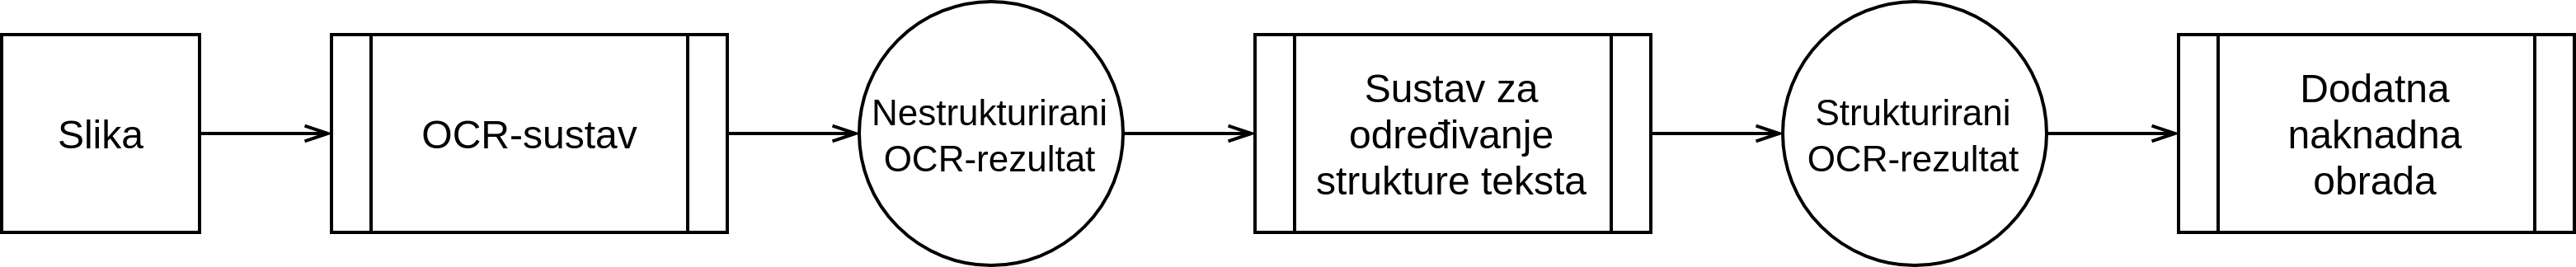
\includegraphics[width=\textwidth]{images/sustav-01.png}
    \caption{Suradnja OCR-sustava i sustava za određivanje strukture teksta.}
    \label{fig:sustav-01}
\end{figure}

U kontekstu određivanja strukture teksta na temelju položaja pojedinih znakova,
radi preglednije analize, razmatramo OCR-sustav koji nema
korak naknadne obrade. Nakon završetka klasifikacije OCR-sustav posjeduje
nestrukturirani OCR-rezultat u kojemu se nalaze svi segmentirani i
klasificirani znakovi. Takav
nestrukturirani OCR-rezultat prosljeđuje se sustavu za određivanje strukture
teksta na naknadnu obradu.
U praksi je sustav za određivanje strukture teksta sastavni dio naknadne obrade OCR-sustava, međutim, u ovom završnom radu ćemo razdvojiti ta dva sustava
radi preglednije analize njihove suradnje.

Sustav za određivanje strukture teksta na temelju položaja pojedinih znakova
(u daljnjem tekstu: \emph{Sustav}) na ulaz od OCR-sustava prima
nestrukturirani OCR-rezultat koji u sebi sadrži sve znakove koje je OCR-sustav
prepoznao. Za svaki znak u OCR-rezultatu znamo sljedeće informacije:
\begin{itemize}
    \item[$\bullet$] $x$ - horizontalnu poziciju gornjeg lijevog kuta,
    \item[$\bullet$] $y$ - vertikalnu poziciju gornjeg lijevog kuta,
    \item[$\bullet$] $width$ - širinu znaka,
    \item[$\bullet$] $height$ - visinu znaka i
    \item[$\bullet$] $value$ - Unicode vrijednost znaka.
\end{itemize}

Izlaz sustava je strukturirani OCR-rezultat u kojemu su znakovi
grupirani u linije, a unutar svake linije su riječi odvojene znakom
bjeline. Strukturirani OCR-rezultat se zatim prosljeđuje dodatnim naknadnim
obradama koje ovise o problemu koji se rješava i u ovom završnom radu o njima
neće biti riječi. Slika \ref{fig:sustav-01} prikazuje vizualizaciju navedenih
suradnji.

U skolpu ovog završnog rada potrebno je razviti sustav za određivanje strukture
teksta koji će rješavati problem određivanja strukture teksta na računima iz
trgovine i sadržaja iz knjga. Stup podataka za testiranje
sustava biti će detaljno objašnjen u odjeljku
\ref{sec:skup-padataka-za-testiranje}.

Slika \ref{fig:book-example-02} prikazuje vizualizaciju rezultata OCR-sustava
koji nam je za svaki znak vratio omeđujući pravokutnik (označeno plavom bojom) i
vrijednost znaka odnosno klasu kojoj znak pripada.
Slike \ref{fig:receipt-example-01} i \ref{fig:book-example-01} također prikazuju
vizualizaciju rezultata OCR sustava i primjere s kakvim će se sustav za
određivanje strukture teksta koji razvijamo susresti.

Primjer pojednostavljenog (detaljnije u odjeljku
\ref{sec:skup-padataka-za-testiranje}) nestrukturiranog OCR-rezultata u formatu
JSON koji će sustav za određivanje strukture teksta dobiti kao svoj ulaz
prikazan je isječkom \ref{lst:ocr-result-json-01}. Ulazni nestrukturirani
OCR-rezultat u formatu JSON uvijek se sastoji od jedne linije u koju
su smješteni svi segmentirani i klasificirani znakovi u nasumičnim redosljedom.

\begin{figure}[htb]
    \centering
    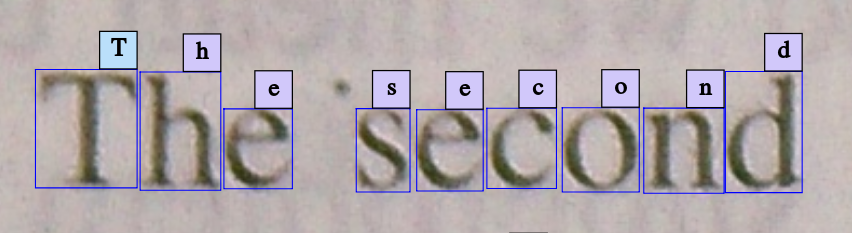
\includegraphics[width=\textwidth]{images/book-example-02.png}
    \caption{Vizualizacija OCR-rezultata.}
    \label{fig:book-example-02}
\end{figure}

\begin{lstlisting}[
    caption={Pojednostavljeni nestrukturirani OCR-rezultat u formatu JSON.},
    label={lst:ocr-result-json-01},
    firstnumber=1
],
{
    "ocr_result": {
        "lines": [
            {
                "chars": [
                    {
                        "x": 25.95604, "y": 17.30562,
                        "width": 10.64438, "height": 16.60289,
                        "value": 48
                    },
                    {
                        "x": 19.77133, "y": 1.28793,
                        "width": 16.07777, "height": 10.76925,
                        "value": 77
                    },
                    {
                        "x": 5.50248, "y": 2.84320,
                        "width": 12.13375, "height": 15.60966,
                        "value": 73
                    },
                    {
                        "x": 3.19550, "y": 19.67606,
                        "width": 14.94088, "height": 20.78798,
                        "value": 91
                    },

                ]
            }
        ]
    }
}
\end{lstlisting}








\section{Željena funkcionalnost}
\label{sec:željena-funkcionalnost}
Od sustava se očekuje da za dobiveni nestrukturirani OCR-rezultat u formatu
JSON vrati novi strukturirani OCR-rezultat u istom formatu koji će znakove
grupirati u linije i koji će unutar linija biti poredani s lijeva na desno.
Također, linije moraju biti sortirane tako da se najviša linija u dokumentu
nalazi na prvom mjestu.

Osim grupiranja linija od sustava se očekuje da između dva znaka, gdje smatra da
završava prethodna i započinje nova riječ, ubaci novi znak bjeline čija je
vrijednost \engl{value} $32$ dok ostale informacije mogu biti prozivoljne.
Dodatan zahtjev je da sustav sve grupirane linije smjesti u jedan blok.
Detaljnije o blokovima će biti opisano u pododjeljku
\ref{subsec:ulazne-datoteke}.

Isječak \ref{lst:ocr-result-json-02} prikazuje primjer izlaza iz sustava za dani
ulaz iz isječka \ref{lst:ocr-result-json-01}. Sustav je znakove grupirao u dvije
linije i između prvog i zadnjeg znaka u drugoj liniji je ubacio znak bjeline.
Vrijednost znaka bjeline je zahtijevana vrijednost $32$. Ostale informacije
znaka bjeline mogle su biti proizvoljne, međutim, sustav im je dodijelio
sljedeće smislenije vrijednosti:\begin{itemize}
    \item[$\bullet$] $x$ - horizontalna pozicija gornjeg desnog kuta lijevog
                           znaka,
    \item[$\bullet$] $y$ - vertikalna pozicija gornjeg lijevog kuta desnog
                           znaka,
    \item[$\bullet$] $width$ - horizontalna udaljenost između gornjeg desnog
                               kuta lijevog znaka i gornjeg lijevog kuta desnog
                               znaka,
    \item[$\bullet$] $height$ - visina lijevog znaka.
\end{itemize}

Pod \emph{lijevi znak} podrazumijeva se na znak koji se nalazi prije znaka
bjeline, a pod \emph{desni znak} podrazumijeva se na znak koji se nalazi nakon
znaka bjeline.

\begin{lstlisting}[
    caption={Izlaz iz sustava za određivanje strukture teksta u formatu JSON.},
    label={lst:ocr-result-json-02},
    firstnumber=1
]
{
    "ocr_result": {
        "lines": [
            {
                "chars": [
                    {
                        "x": 5.50248, "y": 2.84320,
                        "width": 12.13375, "height": 15.60966,
                        "value": 73
                    },
                    {
                        "x": 19.77133, "y": 1.28793,
                        "width": 16.07777, "height": 10.76925,
                        "value": 77
                    }
                ]
            },
            {
                "chars": [
                    {
                        "x": 3.19550, "y": 19.67606,
                        "width": 14.94088, "height": 20.78798,
                        "value": 91
                    },
                    {
                        "x": 18.13638, "y": 19.67606,
                        "width": 7,81966, "height": 20.78798,
                        "value": 32
                    }
                    {
                        "x": 25.95604, "y": 17.30562,
                        "width": 10.64438, "height": 16.60289,
                        "value": 48
                    }
                ]
            }
        ]
    }
}
\end{lstlisting}








\section{Skup podataka za testiranje}
\label{sec:skup-padataka-za-testiranje}
Skup podataka za testiranje (u daljnjem tekstu: \emph{podatci})
sustava sastoji se od slika, ulaznih datoteka u formatu JSON i
očekivanih izlaznih datoteka. U sklopu ovog završnog rada razvijeni sustav za
određivanje strukture teksta rješavati će problem određivanja strukture teksta
na računima iz trgovine i sadržaja iz knjiga.




\subsection{Slike}
\label{subsec:slike}
Podatci za testiranje sustava sadrže $100$ slika računa (primjer na slici
\ref{fig:receipt-example-04}) i $34$ slike sadržaja iz knjiga (primjer na slici
\ref{fig:book-example-03}).

\begin{figure}[htb]
    \centering
    \captionsetup{justification=centering,margin=2cm}
    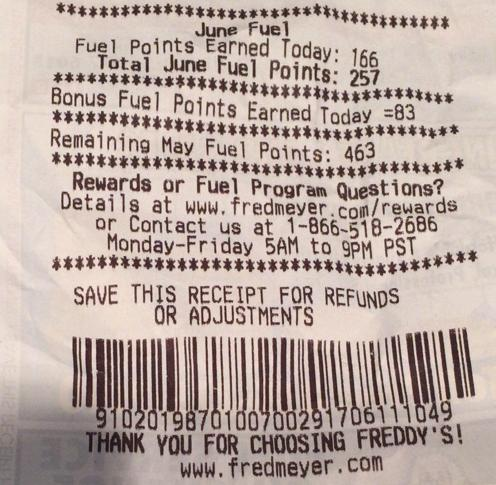
\includegraphics[height=8cm]{images/receipt-example-04.jpg}
    \caption{Primjer slike računa iz trgovine.}
    \label{fig:receipt-example-04}
\end{figure}

\begin{figure}[htb]
    \centering
    \captionsetup{justification=centering,margin=2cm}
    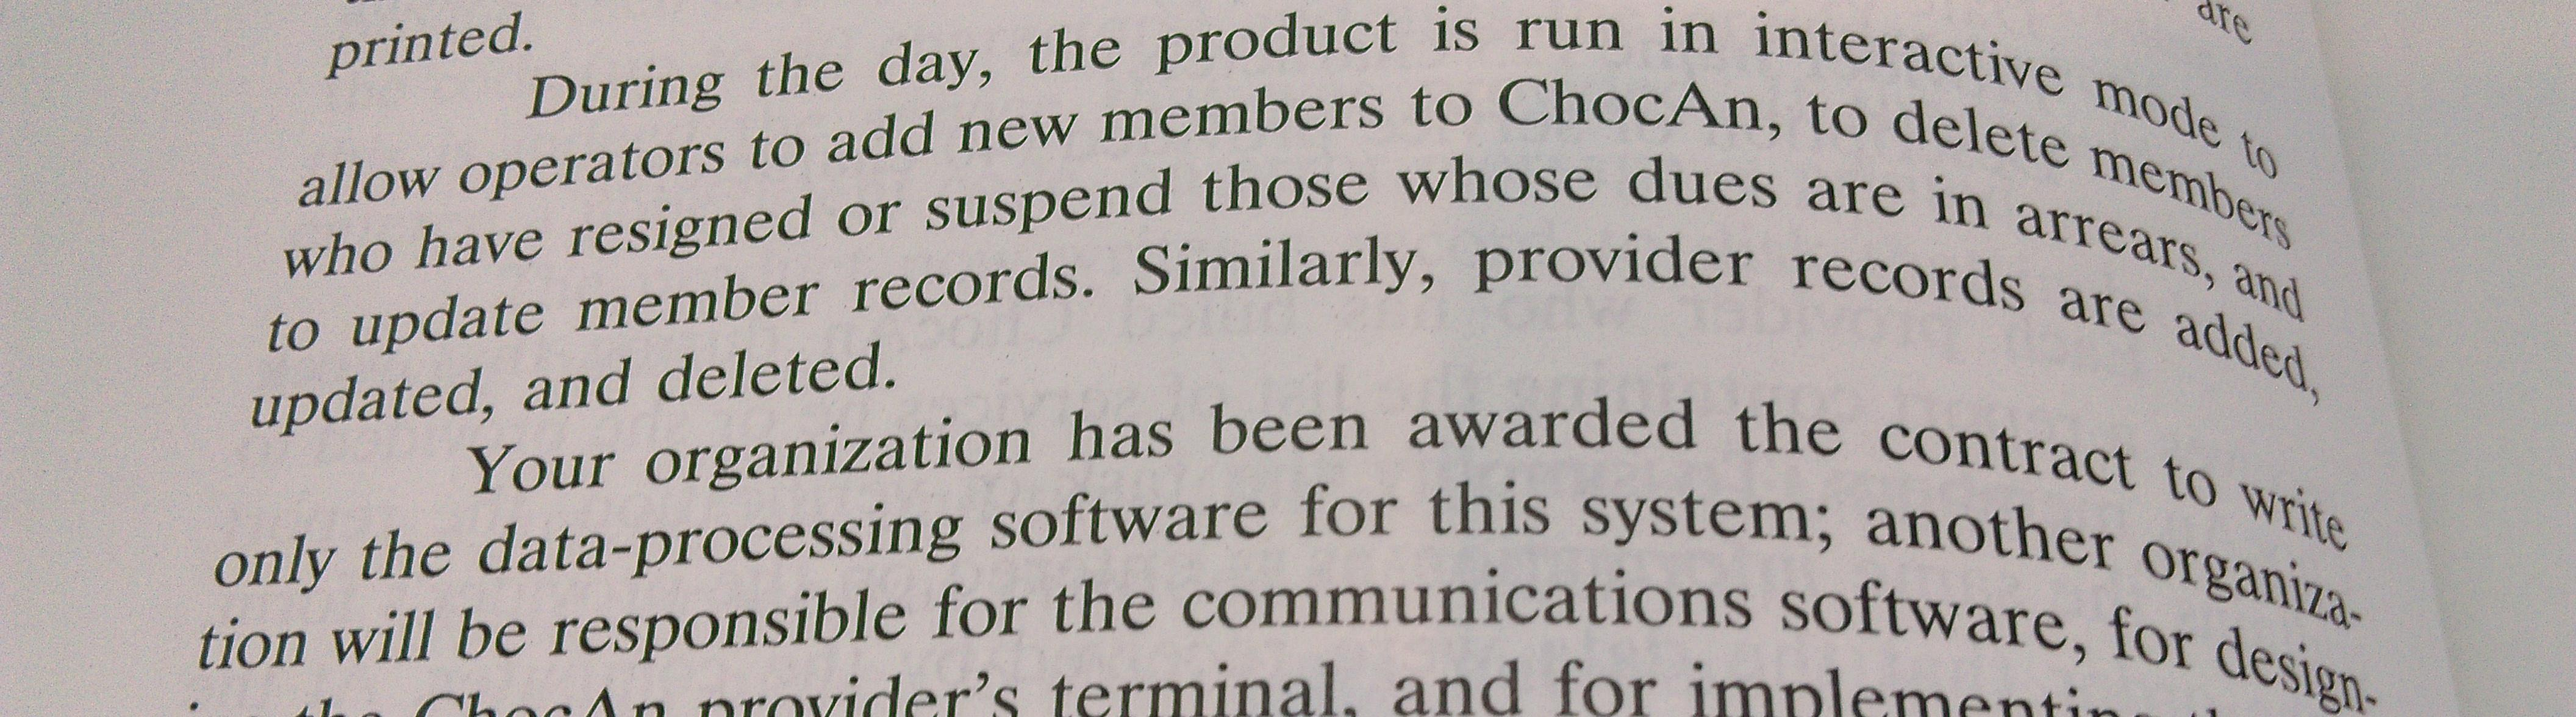
\includegraphics[width=\textwidth]{images/book-example-03.jpg}
    \caption{Primjer slike sadržaja iz knjige.}
    \label{fig:book-example-03}
\end{figure}

Svaki znak na svakoj slici je \textbf{ručno} označen i klasificiran. Na slikama
računa iz trgovine označeno je ukupno $85068$ znakova, a na slikama sadržaja iz
knjiga označeno je ukupno $25092$ znaka. Ručno označeni podatci oponašaju
nestrukturirane OCR-rezultate koji su ulaz u sustav za određivanje strukture
teksta.

Omeđujući pravokutnici označenih znakova predstavljaju područje koje označeni
znak zauzima na slici. Stranice omeđujućih pravokutnika su uvijek paralelne sa
rubovima slike. Slika \ref{fig:book-example-04} prikazuje isječak slike,
sadržaja iz knjige, na kojoj su znakovi ukošeni, a stranice njihovih omeđujućih
znakova paralelne su sa rubovima slike. Možemo uočiti kako je moguće da se dva
susjedna omeđujuća pravokutnika preklapaju.

\begin{figure}[htb]
    \centering
    \captionsetup{justification=centering,margin=2cm}
    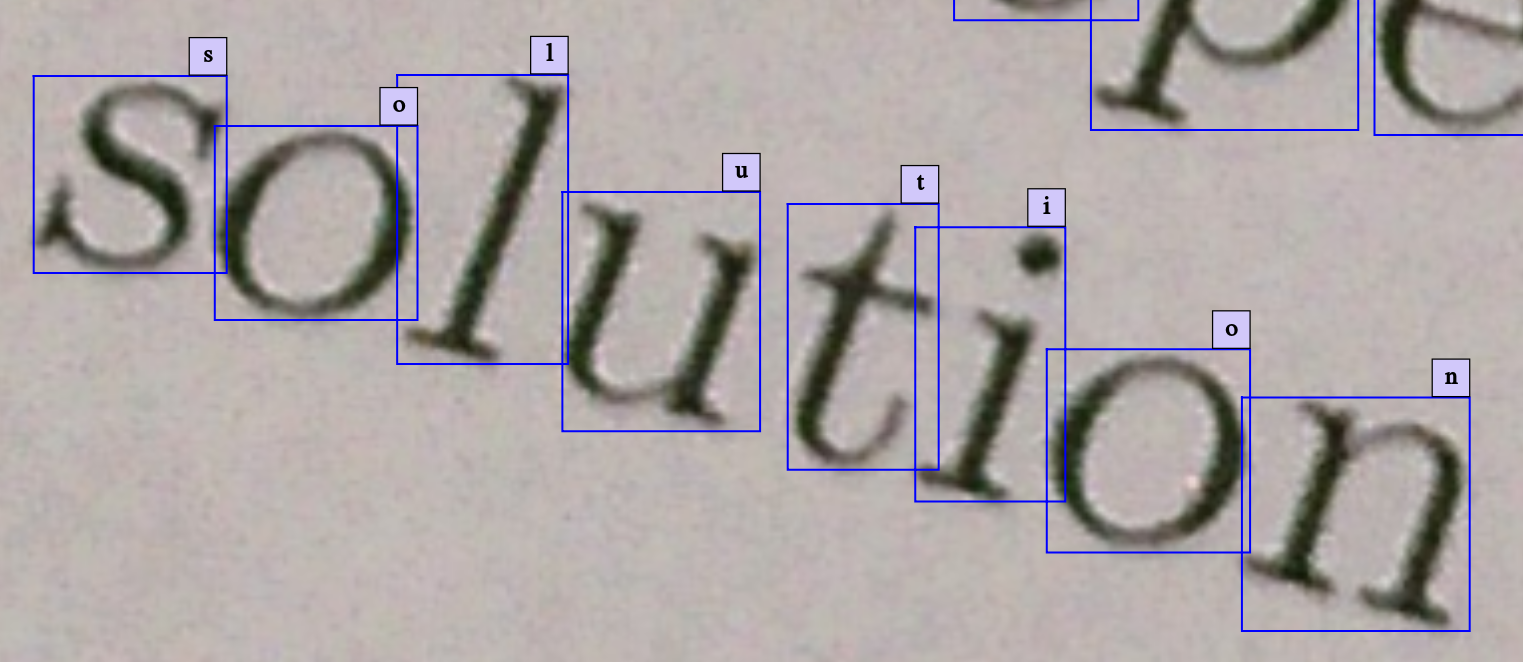
\includegraphics[width=\textwidth]{images/book-example-04.png}
    \caption{Primjer slike s kosim tekstom.}
    \label{fig:book-example-04}
\end{figure}




\subsection{Ulazne datoteke}
\label{subsec:ulazne-datoteke}
Slike opisane u \ref{subsec:slike} \textbf{ne predstavljaju} ulaz u sustav za
određivanje strukture teksta. Nakon označavanja slika podatci o označavanju
svake slike se izvoze i pohranjuju u datoteke u JSON formatu. Datoteke u JSON
formatu predstavljaju nestrukturirani OCR-rezultat i ulaz u sustav. Ulazna
datoteka u formatu JSON u kojoj su zapisani podaci o označavanju slike \ref
{fig:receipt-example-04} prikazana je u isječku \ref{lst:ocr-result-json-03}.
Zbog specifičnosti sustava za označavanje slika i načina na koji pohranjuje
informacije o označavanju, svi označeni znakovi bit će smješteni u jednu liniju
u nasumičnom poretku i ta linija će biti smještena u jedan blok. Za svaki znak
dostupna je informacija o Unicode vrijednosti znaka koja je smještena pod
ključem \lstinline{value}. Dodatno, za svaki znak dostupna je informacija o
poziciji i veličini njegovog omeđujućeg pravokutnika \engl{bounding box}. Za
svaki omeđujući pravokutnik poznate su sljedeće informacije:
\begin{itemize}
    \item[$\bullet$] $x$ - horizontalna pozicija gornjeg lijevog kuta,
    \item[$\bullet$] $y$ - vertikalna pozicija gornjeg lijevog kuta,
    \item[$\bullet$] $width$ - širina i
    \item[$\bullet$] $height$ - visina.
\end{itemize}

Kako vrijednost $x$ omeđujućeg pravokutnika raste tako je znak bliže desnom rubu
slike. Kako vrijednost $y$ omeđujućeg pravokutnika raste tako je znak bliže
donjem rubu slike. Sve informacije o omeđujućem pravokutniku su vrijednosti iz
skupa nenegativnih realnih brojeva.

Sustav za označavanje slika izvozi još neke dodatne informacije o znakovima i
o označenoj slici. Sve informacije koje nisu ovdje navede mogu se zanemariti.

\begin{lstlisting}[
    caption={
        JSON datoteka s podatcima o označavanju slike
        \ref{fig:receipt-example-04}.
    },
    label={lst:ocr-result-json-03},
    firstnumber=1
]
{
    "ocr_result": {
        "blocks": [
            {
                "lines": [
                    {
                        "chars": [
                            {
                                "value": 83,
                                "bounding_box": {
                                    "x": 4.548218,
                                    "y": 271.68826,
                                    "width": 12.136101,
                                    "height": 22.48648
                                }
                            },
                            {
                                "value": 65,
                                "bounding_box": {
                                    "x": 4.244385,
                                    "y": 247.67685,
                                    "width": 12.59581,
                                    "height": 21.750519
                                }
                            },
                            // ostalih 388 znakova
                        ]
                    }
                ]
            }
        ]
    }
}
\end{lstlisting}


\subsubsection{Izlaz iz sustava za određivanje strukture teksta}
U odjeljku \ref{sec:željena-funkcionalnost} navedeni su zahtjevi sustava i
opisan je pojednostavljeni format izlaza iz sustava. Od sustava se očekuje da
rezultat nakon određivanja strukture teksta prikaže u istom formatu u kojemu je
prikazan ulaz u sustav opisan u ovom odjeljku. Sve grupirane linije potrebno je
smjestiti u jedan blok. Sustav ne treba isporučiti informacije koje su se mogu
zanemariti na ulazu.




\subsection{Očekivane izlazne datoteke}
\label{subsec:očekivane-izlazne-datoteke}
Očekivane izlazne datoteke predstavljaju ispravni strukturirani tekstualni
sadržaj sa slike. Isječak \ref{lst:txt-result-04} predstavlja ispravni
strukturirani tekstualni sadržaj računa sa slike \ref{fig:receipt-example-04}.
Uočimo da u tekstualnom sadržaju ne postoje bjeline prije početka linije koje
postoje u sadržaju na slici. Osim toga, višestruke bjeline u sadržaju na slici
predstavljene su točno jednom bjelinom u tekstualnom sadržaju u datoteci.

\begin{lstlisting}[
    caption={
        Tekstualni sadržaj slike \ref{fig:receipt-example-04}.
    },
    label={lst:txt-result-04},
    firstnumber=1
]
POINTS TO $35 REWARD 8770
BALANCE REWARDS ACCT # *********2463
OPENING BALANCE 20820
EVERYDAY POINTS - RETAIL 410
CLOSING BALANCE 21230
*****************************************
Walgreens 01875
ACCT 7681
SEQUENCE 1875220350
PAYMENT FROM PRIMARY
Get the flu shot that helps provide
a lifesaving vaccine to a child in need
Get a Shot. Give a Shot.® It's that easy
Learn more at the pharmacy.
\end{lstlisting}








\section{Korištenje skupa podataka za testiranje}
\begin{figure}[htb]
    \centering
    \captionsetup{justification=centering,margin=2cm}
    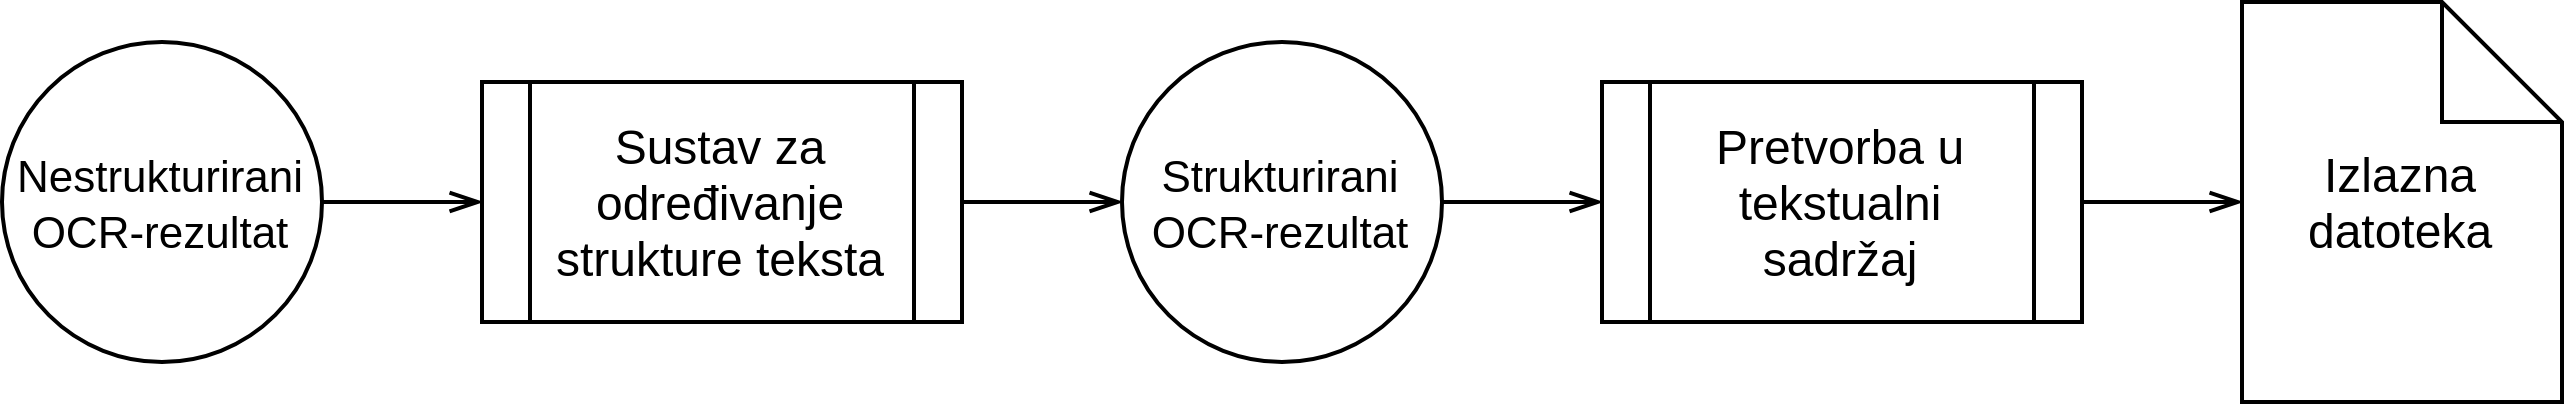
\includegraphics[width=\textwidth]{images/sustav-02.png}
    \caption{
        Postupak dobivanja izlazne datoteke iz strukturiranog OCR-rezultata.
    }
    \label{fig:sustav-02}
\end{figure}
Slika \ref{fig:sustav-02} prikazuje postupak dobivanja izlazne datoteke iz
strukturiranog OCR-rezultata kojeg je vratio sustav za određivanje strukture
teksta. Ulaz u sustav je ulazna datoteka u formatu JSON koja predstavlja
nestrukturirani OCR-rezultat kao što je opisano u pododjeljku
\ref{subsec:ulazne-datoteke}.
Izlaz iz sustava je strukturirani OCR-rezultat u formatu JSON u kojemu se nalaze
znakovi grupirani u linije i gdje su između riječi ubačeni znakovi bjeline.
Strukturirani OCR-rezultat u formatu JSON potrebno je pretvoriti u izlaznu
datoteku koja predstavlja strukturirani tekstualni sadržaj u formatu opisanom u
pododjeljku \ref{subsec:očekivane-izlazne-datoteke} koji se onda
uspoređuje sa očekivanim izlaznim datotekama dostupnim u skupu podataka za
testiranje. Isječak \ref{lst:ocr-result-to-txt} prikazuje pseudokôd algoritma
za ispis OCR-rezultata na standradni izlaz.

\begin{lstlisting}[
    caption={Pseudokôd algoritma za ispis OCR-rezultata na standardni izlaz.},
    label={lst:ocr-result-to-txt},
    morekeywords={def,for,end,if,else,return},
    firstnumber=1
],
def ispisi(ocrRezultat)
  for linija u ocrRezultat.linije
    for znak u linija
      print(znak.value)
    end
    print("\n")
  end
end
\end{lstlisting}

Metode usporedbe izlaznih datoteka dobivenih iz strukturiranih OCR-rezultata i
očekivanih izlaznih datoteka iz skupa podataka za testiranje biti će objašnjene
u odjeljku.
















\chapter{Algoritmi za određivanje strukture teksta}
Sustav za određivanje strukture teksta podijeljen je u dva podsustava:
\textbf{sustav za određivanje linija} i \textbf{sustav za rastavljanje riječi}.
Slika \ref{fig:sustav-02} prikazuje navedene komponente sustava i njihovu
suradnju. Ulaz u sustav za određivanje linija je nestrukturirani OCR-rezultat
dobiven od OCR-sustava koji je ujedno i ulaz u sustav za određivanje strukture
teksta. Izlaz iz sustava za određivanje linija je OCR-rezultat
u kojemu su znakovi grupirani u linije kojima pripadaju. Izlaz
iz sustava za određivanje linija je ulaz u sustav za rastavljanje riječi koji
u svakoj liniji ubacuje na odgovarajuća mjesta znakove bjeline koji odvajaju
riječi. Izlaz iz sustava za rastavljanje riječi je ujedno i izlaz iz sustava
za određivanje strukture teksta.
\begin{figure}[htb]
    \centering
    \captionsetup{justification=centering,margin=2cm}
    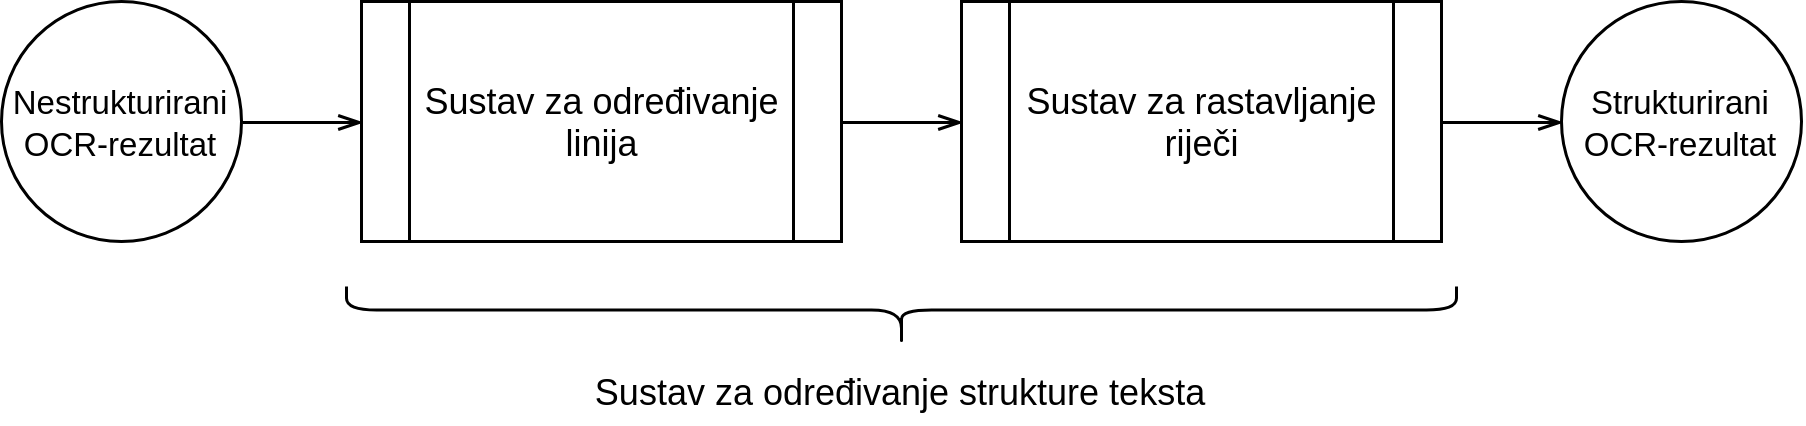
\includegraphics[width=\textwidth]{images/sustav-03.png}
    \caption{
        Komponente sustava za određivanje strukture teksta.
    }
    \label{fig:sustav-03}
\end{figure}

U formalnoj definiciji i analizi algoritama koristit ćemo sljedeće oznake:
\begin{itemize}
    \item[$\bullet$] $C$ - označava skup svih znakova u OCR-rezultatu,
    \item[$\bullet$] $A$ i $B$ - označavaju pojedini znak u OCR-rezultatu koji ima svoju širinu $A_w$, visinu $A_h$, horizontalnu $x$ poziciju lijevog
    gornjeg kuta $A_x$, vertikalnu $y$ poziciju lijevog gornjeg kuta $A_y$ i
    Unicode vrijednost $A_v$,
    \item[$\bullet$] $v$ - označava Unicode vrijednost,
    \item[$\bullet$] $L$ - označava skup svih linija u OCR-rezultatu,
    \item[$\bullet$] $l$ i $k$ - označavaju pojedinu liniju u OCR-rezultatu,
    \item[$\bullet$] $l_{-i}$ - označava $i$-ti znak od kraja u liniji $l$, pa
    tako npr.\ $l_{-1}$ označava zadnji znak u liniji $l$,
    \item[$\bullet$] $l_i$ - označava $i$-ti znak od početka u liniji $l$, pa
    tako npr.\ $l_1$ označava prvi znak u liniji $l$.
\end{itemize}

Linije također smatramo skupovima pa će $|l|$ označavati duljinu linije $l$,
a za znak $A$ reći ćemo da pripada liniji $l$ ako vrijedi $A \in l$.

Za dva znaka $A$ i $B$ kažemo da su jednaki ako i samo ako vrijedi:
\[
A = B \iff
A_w = B_w \land A_h = B_h \land A_x = B_x \land A_y = B_y \land A_v = B_v
\]

Definirajmo unaprijed nekoliko horizontalnih udaljenosti između dva znaka $A$ i
$B$:
\begin{align}
d(A, B) &= |\max(A_x, B_x) - \min(A_x + A_w, B_x + B_w)| \\
d_l(A, B) &= |A_x - B_x| \\
d_c(A, B) &= |A_x + \frac{A_w}{2} - (B_x + \frac{B_w}{2})| \\
\hat{d}(A, B) &= \frac{d(A, B)}{\min(A_w, B_w)} \\
\hat{d_l}(A, B) &= \frac{d_l(A, B)}{\min(A_w, B_w)} \\
\hat{d_c}(A, B) &= \frac{d_c(A, B)}{\min(A_w, B_w)}
\end{align}

Udaljenost $d$ predstavlja udaljenost između desnog ruba lijevog znaka i
lijevog ruba desnog znaka. Udaljenost $d_l$ predstavlja udaljenost lijevih
rubova znakova, a udaljenost $d_c$ predstavlja udaljenost centara znakova.
Udaljenosti $\hat{d}$, $\hat{d_l}$ i $\hat{d_c}$ predstavljaju normalizirane
udaljenosti $d$, $d_l$ i $d_c$.

S ovako definiranim oznakama možemo npr.\ definirati skup svih znakova koji
imaju Unicode vrijednost jednaku $v$:
\[ S(v) = \left\{A \vert A \in C, A_v = v\right\} \]

U nastavku ovog poglavlja koristiti ćemo navedene oznake u formalnoj definiciji
algoritama za određivanje linija i algoritama za rastavljanje riječi.








\section{Algoritmi za određivanje linija}
\label{sec:algoritmi-za-odredivanje-linija}
Algoritmi za određivanje linija trebaju na temelju omeđujućih pravokutnika
svakog znaka znakove grupirati u linije. Slika \ref{fig:line-semgentation-01}
predstavlja vizualizaciju očekivanog rezultata algoritma za određivanje linija.

\begin{figure}[htb]
    \centering
    \captionsetup{justification=centering,margin=2cm}
    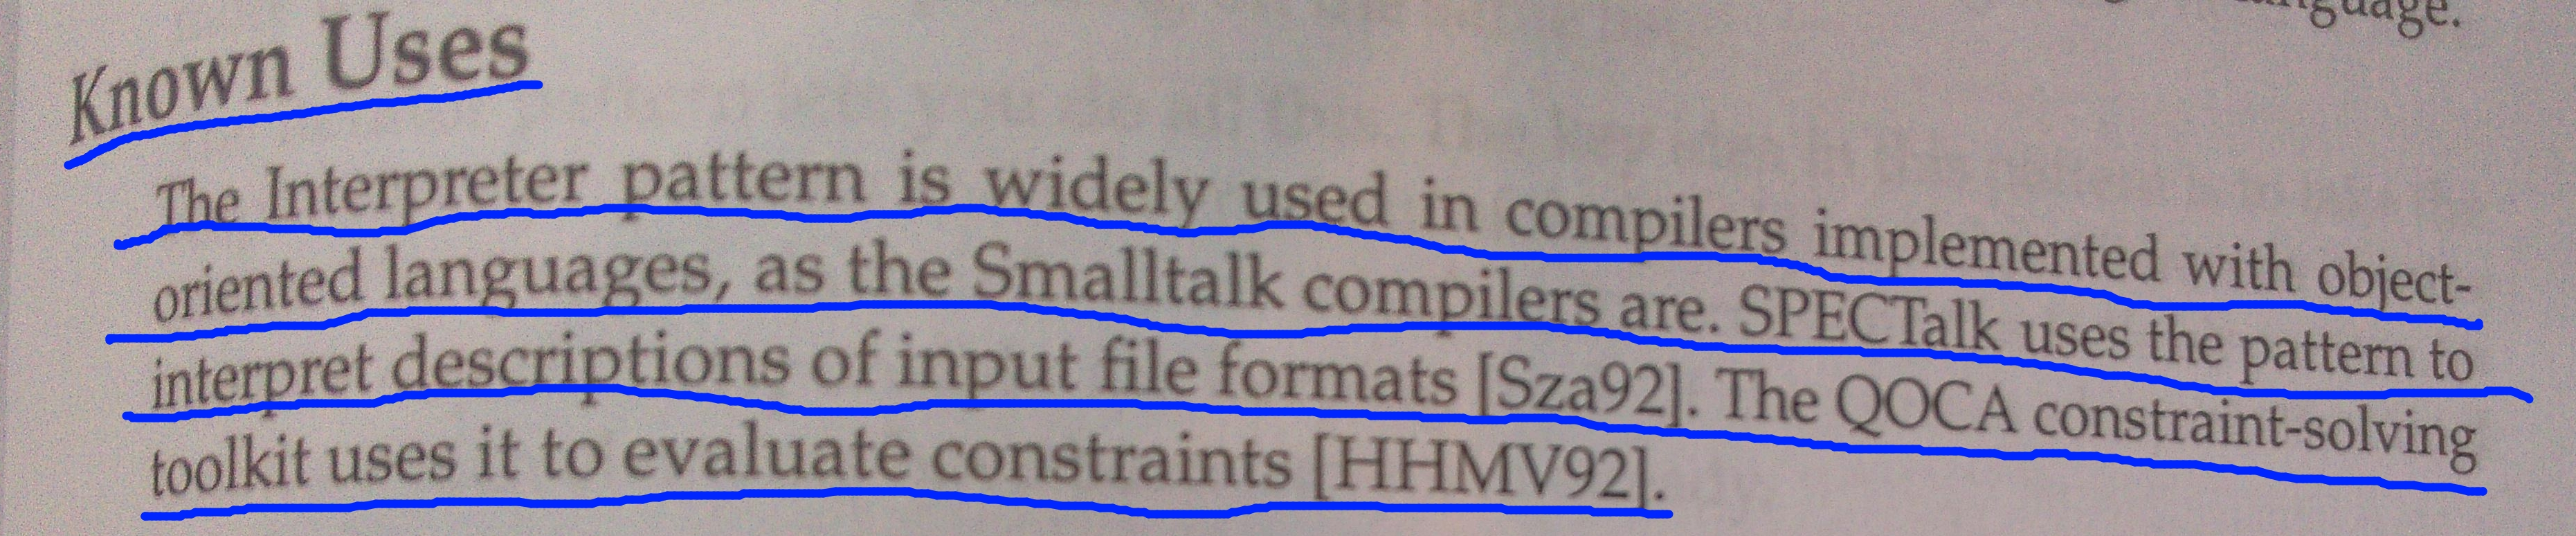
\includegraphics[width=\textwidth]{images/line-segmentation-01.jpg}
    \caption{
        Vizualizacija detektiranih linija u sadržaju iz knjige.
    }
    \label{fig:line-semgentation-01}
\end{figure}

Algoritam na ulazu prima nestrukturirani OCR-rezultat koji je ujedno i ulaz u
sustav za određivanje strukture teksta. Izlaz iz algoritma je OCR-rezultat u
kojemu su znakovi grupirani u linije, sortirani s lijeva na desno i u kojemu
su linije sortirane tako da se najviša linija na slici nalazi na prvom mjestu.




\subsection{Algoritam temeljen na maksimalnom preklapanju znakova}
Algoritam za određivanje linija na temelju maksimalnog preklapanja znakova
(u daljnjem tekstu: \emph{algoritam}) temelji se na pretpostavci da dva susjedna
znaka koja se nalaze u istoj liniji ostvaruju maksimalno vertikalno preklapanje.
Vertikalno preklapanje \textit{overlap} dva znaka $A$ i $B$ definiramo izrazom:

\begin{equation}
\label{eq:overlap}
\textit{overlap}(A, B) =
\frac{\max(0, \min( A_y + A_h, B_y + B_h ) - \max( A_y, B_y ))}{\min(A_h, B_h)}
\end{equation}

Na početku svog rada algoritam uzlazno sortira sve znakove po horizontalnoj $x$
vrijednost, zatim iterira po svakom znaku i konstruira linije gledajuću s kojom
linijom promatrani znak ostvaruje maksimalno preklapanje. Preklapanje s linijom
definira se kao preklapanje sa zadnjim znakom u toj liniji. Promatrani znak
pripadne onoj liniji s kojom ostvari maksimalno preklapanje:

\begin{equation}
\label{eq:overlap-01}
l_{max} = \argmax_{l \in L}\left\{\textit{overlap}(A, l_{-1})\right\}
\end{equation}

Ako je znak s nekom linijom ostvario preklapanje u vrijednosti $0$ tada on
postaje početak nove linije i u skup $L$ dodaje se ta nova linija. Na ovaj
način algoritam zapravo konstruira linije i skup $L$ koji je na početku
prazan.


\subsubsection{Rješavanje problema valovitih linija}
Budući da linije u sadržaju skupa podataka kojeg promatramo mogu biti valovite
(slika \ref{fig:aligner-01}), ponekad je poželjno izmjeriti preklapanje ne samo
sa zadnjim znakom u liniji nego i sa zadnjih nekoliko:
\begin{equation}
\label{eq:overlap-02}
l_{max} = \argmax_{l \in L,\ i \in [1, \min(|l|, c_1)]}\left\{\textit{overlap}(A, l_{-i})\right\}
\end{equation}

Za razliku od izraza \ref{eq:overlap-01} koji uzima u obzir samo zadnji znak u
svakoj liniji, izraz \ref{eq:overlap-02} uzet će u obzir zadnjih
$\min(|l|, c_1)$
znakova u svakoj liniji, gdje $c_1$ predstavlja \textbf{parametar algoritma}. Eksperimentalno je utvrđeno da vrijednost parametra $c_1 = 1$ ostvaruje najbolje rezultate na sadržaju s računima iz trgovine, a da vrijednost parametra $c_1 = 2$ ostvaruje najbolje rezultate na sadržaju iz knjiga.

Slika \ref{fig:aligner-01} prikazuje kako znak \lstinline{=} na desnoj strani
crvenog pravokutnika ostvaruje maksimalno preklapanje sa znakom \lstinline{=}
na lijevoj strani crvenog pravokutnika koji nije zadnji znak u liniji u tom
trenutku.
\begin{figure}[htb]
    \centering
    \captionsetup{justification=centering,margin=2cm}
    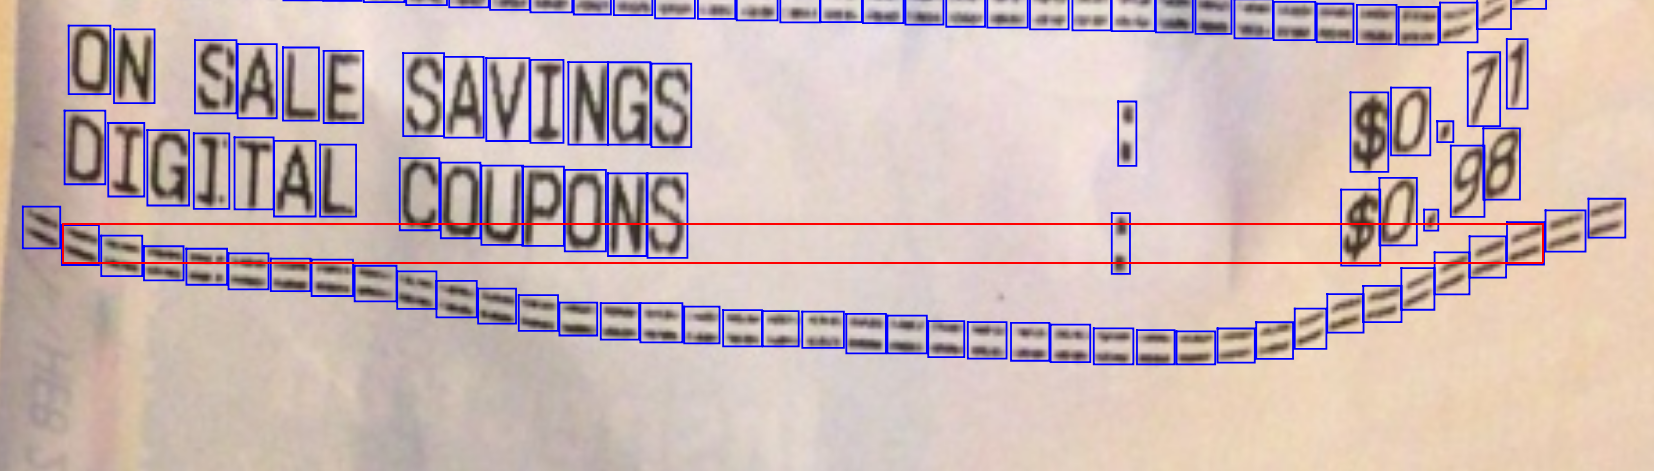
\includegraphics[width=\textwidth]{images/aligner-01.png}
    \caption{Valovite linije otežavaju određivanje linija.}
    \label{fig:aligner-01}
\end{figure}


\subsubsection{Rješavanje problema preklapanja početaka dviju linija}
Slika \ref{fig:overlap-01} prikazuje kako je moguće preklapanje početaka dviju
linija. Tako znakovi \lstinline{0} i \lstinline{D}
ostvaruju nezanemarivo preklapanje čija će posljedica biti krivo određene
linije. Kako bismo uspješno detektirali ovakve slučajeve uvodimo dodatan uvijet
koji će odlučiti hoće li promatrani znak pripasti liniji s kojom ostvaruje
maksimalno preklapanje:

\begin{equation}
\label{eq:overlap-03}
\max_{i \in [1, \min(|l_{max}|, c_1)]}\left\{\textit{overlap}(A, l_{max_{-i}})\right\} > c_2
\end{equation}

\begin{figure}[htb]
    \centering
    \captionsetup{justification=centering,margin=2cm}
    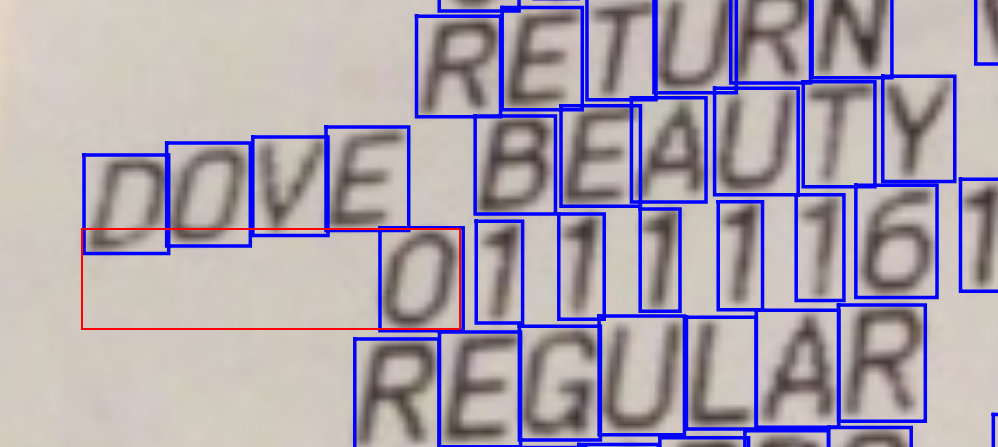
\includegraphics[width=\textwidth]{images/overlap-01.png}
    \caption{Preklapanje početaka dviju linija.}
    \label{fig:overlap-01}
\end{figure}

Nakon što smo izrazom \ref{eq:overlap-02} odredili s kojom linijom promatrani
znak ostvaruje maksimalno preklapanje trebamo provjeriti zadovoljava li iznos
tog preklapanja uvijet naveden izrazom \ref{eq:overlap-03}. Uvodimo novi
parametar algoritma $c_2$ koji predstavlja donju granicu preklapanja koju znak
mora ostvariti s linijom da bi joj se pripojio. Eksperimentalno je utvrđeno da
vrijednost parametra $c_2 = 0,13$ ostvaruje najbolje rezultate na sadržaju s
računima iz trgovine, a da vrijednost parametra $c_2 = 0,05$ ostvaruje najbolje
rezultate na sadržaju iz knjiga.

\begin{figure}[htb]
    \centering
    \captionsetup{justification=centering,margin=2cm}
    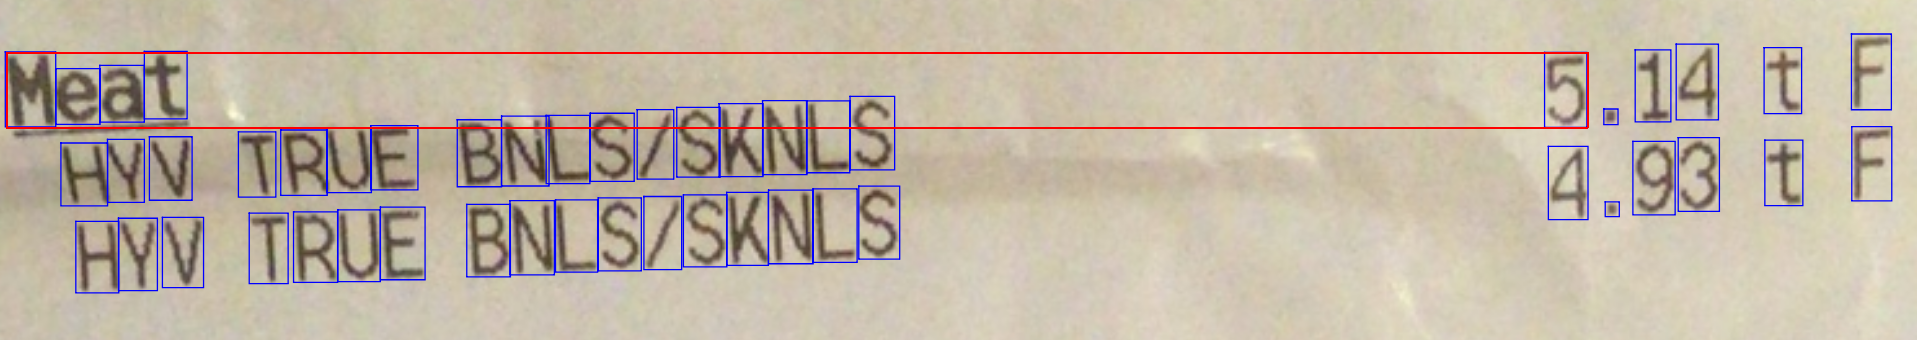
\includegraphics[width=\textwidth]{images/overlap-02.png}
    \caption{Lažno pozitivno preklapanje}
    \label{fig:overlap-02}
\end{figure}


\subsubsection{Rješavanje problema lažno pozitivnog preklapanja}
Slika \ref{fig:overlap-02} prikazuje slučaj kada znak pripadne krivoj liniji
zato jer s njom ostvaruje maksimalno preklapanje zbog zakrivljenosti slike i
sadržaja. U ovom primjeru znak \lstinline{5} pripasti će prvoj liniji
\lstinline{Meat}, a trebao bi pripasti drugoj liniji. Promatrajući skup
podataka za koji rješavamo problem zaključili smo kako uvijek treba dati
prednost onoj liniji čiji je zadnji znak bliži znaku kojeg promatramo. Tako će
u primjeru sa slike \ref{fig:overlap-02} znak \lstinline{5} pripasti drugoj
liniji zato jer je njezin zadnji znak bliži znaku \lstinline{5} nego znak
\lstinline{t} iz prve linije i zato jer s zadnjim znakom u drugoj liniji ipak
postiže nezanemarivo preklapanje.

Za rješavanje ovog problema definirat ćemo dvije funkcije (slika
\ref{fig:function-01})
koje koriste dva nova parametra algoritma $c_3$ i $c_4$:

\begin{align}
f_1(x) &= \frac{1}{1 + c_3 \cdot x} \\[10pt]
f_2(x) &= 1 + \frac{c_4 \cdot x}{1 + c_4 \cdot x}
\end{align}

\begin{figure}[htb]
    \centering
    \captionsetup{justification=centering,margin=2cm}
    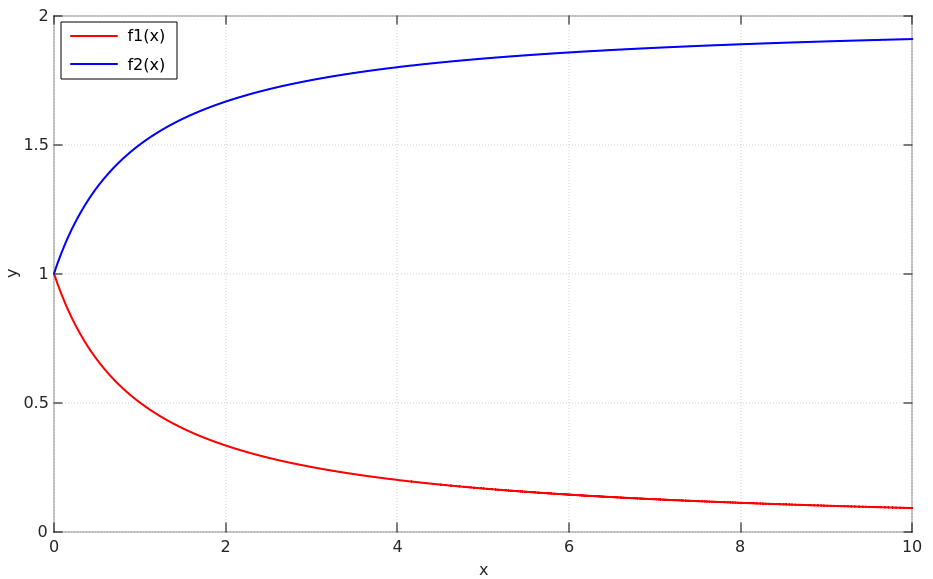
\includegraphics[width=\textwidth]{images/function-01.png}
    \caption{
        Grafovi funkcije $f_1$ (crveno) i funkcije $f_2$ (plavo) za parametre
        $c_3 = c_4 = 1$.
    }
    \label{fig:function-01}
\end{figure}

Ideja je da koristimo navedene funckije $f_1$ i $f_2$ kako bismo linijama
olakšali odnosno otežali postizanje preklapanja u ovisnosti o udaljenosti između
njihovih zadnjih znakova. Recimo da u smo u postupku traženja maksimalnog
preklapanja u jednom trenutku ostvarili maksimalno preklapanje s linijom $l$
iznosa $p_l$. S idućom linijom $k$ izmjerimo preklapanje $p_k$. Da bi linija
$k$ postigla novo maksimalno preklapanje sa promatranim znakom mora vrijediti
$p_k > p_l$. Međutim, recimo da smo uočili da je zadnji znak linije $k$
bliži promatranom znaku nego zadnji znak linije $l$. Koristeći navedenu
opservaciju možemo liniji $k$ olakšati postizanje novog maksimalnog
preklapanja tako da ostvareno preklapanje linije $l$ umanjimo za neki iznos.
Budući da je zadnji znak linije $k$ bliži promatranom znaku novi uvijet koji
linija $k$ mora zadovoljiti da bi ju smatrali novim maksimalnim preklapanjem
glasi:

\begin{equation}
p_k > p_l \cdot f_1(\hat{d_l}(l_{-1},k_{-1}))
\end{equation}

Funkcija $f_1$ će liniji $k$ pomoći tim više što su zadnji znakovi linija
$l$ i $k$ udaljeniji. Da je zadnji znak linije $k$ bio dalje od
promatranog znaka nego zadnji znak linije $l$ onda bismo liniji $k$ trebali
otežati postizanje novog maksimalnog preklapanja čak i ako vrijedi $p_k > p_l$. U tom slučaju novi uvijet za liniju $k$ glasi:

\begin{equation}
    p_k > p_l \cdot f_2(\hat{d_l}(l_{-1},k_{-1}))
\end{equation}

Funkcija $f_2$ će liniji $k$ otežati tim više što su zadnji znakovi linija
$l$ i $k$ udaljeniji. Eksperimentalno je utvrđeno da vrijednosti parametra
$c_3 = c_4 = 0{,}13$ ostvaruje najbolje rezultate na sadržaju s računima iz
trgovine i na sadržaju iz knjiga.

Nakon što smo svaki znak smjestili u odgovarajuću liniju, linije je potrebno
sortirati uzlazno po $y$ vrijednosti prvih znakova linije. Naime, u početnom
koraku sortiranja znakova po $x$ vrijednosti moguće je da prvi znak
u sortiranim znakovima započinje neku liniju u sadržaju koja nije prva.
Budući da će taj znak u našem algoritmu biti detektiran kao početak nove linije
koju ćemo zatim smjesitit na početak, a ne na mjesto kojem ta linija pripada.

Konačno, pseudokôd algoritma za određivanje linija na temelju maksimalnog
preklapanja znakova prikazan je u isječku. U navedenom isječku funkcije $f_1$ i
$f_2$ implicitno koriste vrijednost $0{,}13$ za parametare $c_3$ i $c_4$.
U pseudokôdu funkcija \lstinline{dln} označava funkciju udaljenosti $\hat{d_l}$.

\begin{lstlisting}[
    caption={Pseudokôd algoritma za određivanje linija.},
    label={lst:algorithm-01},
    morekeywords={def,for,end,if,else,return,new},
    firstnumber=1
],
def odrediLinije(nestrukturiraniOcrRezultat)
  znakovi = sortirajPoX(nestrukturiraniOcrRezultat.sviZnakovi)
  linije = []

  for znak u znakovi
    maxPreklapanje = 0
    linijaSaMaxPreklapanjem = null
    for linija u linije
      p = 0
      tezina = 1
      for i u [0, min(c1, linija.duljina)]
        p = max(p, overlap(znak, linija[-i]))
      end
      if linijaSaMaxPreklapanjem != null
        if linijaSaMaxPreklapanjem[-1].x < linija[-1].x
          tezina = f1(dln(linijaSaMaxPreklapanjem[-1], linija[-1]))
        else
          tezina = f2(dln(linijaSaMaxPreklapanjem[-1], linija[-1]))
        end
      end
      if p > maxPreklapanje * tezina
        maxPreklapanje = p
        linijaSaMaxPreklapanjem = linija
      end
    end

    if maxPreklapanje > c2
      linijaSaMaxPreklapanjem.nadodaj( znak )
    else
      linije.nadodaj([znak])
    end
  end

  sortiraneLinije = sortirajPoY(linije)

  return new OcrRezultat(sortiraneLinije)
end
\end{lstlisting}








\section{Algoritmi za rastavljanje riječi}
Algoritmi za rastavljanje riječi na ulaz primaju OCR-rezultat u kojemu su
znakovi grupirani u linije u prethodnom koraku opisanom u odjeljku
\ref{sec:algoritmi-za-odredivanje-linija}. Zadaća algoritama za rastavljanje
riječi je da između znakova, za koje smatra da su završetak prethodne odnosno
početak iduće riječi, ubaci znak bjeline čija će vrijednost \engl{value} biti
$32$, a ostale informacije mogu biti proizvljne.

U nastavku ovog odjeljka opisati ćemo tri algoritma za rastavljanje riječi:
\begin{itemize}
    \item[$\bullet$] algoritam temeljen na prosječnoj širini znaka
    \item[$\bullet$] algoritam temeljen na prosječnoj relativnoj
                     udaljenosti
    \item[$\bullet$] algoritam temeljen na prosječnoj udaljenosti centara
\end{itemize}



\subsection{Algoritam temeljen na prosječnoj širini znaka}
\label{subsec:algoritam-temeljen-na-prosjecnoj-sirini znaka}
Algoritam temeljen na prosječnoj širini znaka najjednostaviji je od svih
algoritama koje ćemo u ovom odjeljku opisati. Algoritam se temelji na
pretpostavci da je širina razmaka između riječi propocionalna sa prosječnom
širinom znakova u promatranoj liniji. Označimo prosječnu širinu znaka u liniji
$l$ sa $\overline{w_l}$:

\begin{equation}
\overline{w_l} = \frac{\mathlarger{\sum}\limits_{A \in l} A_w}{|l|}
\end{equation}

Sada možemo postaviti uvijet koji će odlučiti treba li ubaciti bjelinu između
dva znaka $A$ i $B$:

\begin{equation}
\label{eq:condition-01}
d(A, B) > \overline{w_l} \cdot c_1
\end{equation}

Parametar $c_1$ je jedini \textbf{parametar algoritma} za koji smo
eksperimentalno utvrdili da najbolje rezultate za sadržaj na računima iz
trgovine ostvaruje vrijednost $0{,}8$, a najbolje rezultate za sadržaj iz knjiga
ostvaruje vrijednost $0{,}44$. Isječak \ref{lst:algorithm-02} prikazuje
pseudokôd algoritma za rastavljanje riječi temeljenog na prosječnoj širini
znaka.

\begin{lstlisting}[
    caption={
        Pseudokôd algoritma za rastavljanje riječi temeljen na
        prosječnoj širini znaka.
    },
    label={lst:algorithm-02},
    morekeywords={def,for,end,if,else,return,while,new},
    firstnumber=1
],
def rastaviRijeci(ocrRezultat)
  for linija u ocrRezultat.linije
    prosjecnaSirina = 0
    for znak u linija
      prosjecnaSirina += znak.width
    end
    prosjecnaSirina /= linija.duljina

    i = 0
    j = 1
    while j < linija.duljina
      udaljenost = d(linija[i], linija[j])
      if udaljenost > prosjecnaSirina * c1
        bjelina = new Znak()
        bjelina.value = 32
        bjelina.x = linija[i].x + linija[i].width
        bjelina.y = linija[i].y
        bjelina.width = udaljenost
        bjelina.height = linija[i].height
        linija.ubaciZnakPrijePozicije(j, znak)
        i += 2
        j += 2
      else
        i++
        j++
      end
    end
  end

  return ocrRezultat
end
\end{lstlisting}

Algoritam prikazan pseudokôdom \ref{lst:algorithm-02} ubacuje znak bjeline
čija je vrijednost jednaka $32$, a ostale informacije su određene na sljedeći
način:
\begin{itemize}
    \item[$\bullet$] $x$ - horizontalna pozicija gornjeg desnog kuta lijevog
                           znaka,
    \item[$\bullet$] $y$ - vertikalna pozicija gornjeg lijevog kuta desnog
                           znaka,
    \item[$\bullet$] $width$ - horizontalna udaljenost između gornjeg desnog
                               kuta lijevog znaka i gornjeg lijevog kuta desnog
                               znaka,
    \item[$\bullet$] $height$ - visina lijevog znaka.
\end{itemize}

Pod \emph{lijevi znak} misli se na znak u liniji na poziciji $i$, a pod
\emph{desni znak} misli se na znak u liniji na poziciji $j$. U liniji $20$
ubacujemo novi znak bjeline prije znaka na poziciji $j$ što
ima za posljedicu pomicanje svih elemenata desno od $j$, uključujući i element
na poziciji $j$, za jedno mjesto udesno.




\subsection{Algoritam temeljen na prosječnoj relativnoj udaljenosti}
Algoritam temeljen na prosječnoj relativnoj udaljenosti temelji se na
pretpostavci da je udaljenost znaka $A$ s vrijednosti \engl{value} $A_v$
proporcionalna s prosječnom udaljenosti koju svi znakovi s
vrijednosti $A_v$ ostvaruju sa svojim susjedima.

Skup svih susjeda znaka $A$ definiramo kao skup svih znakova $B$ koji su
različiti od $A$, koji se nalaze u istoj liniji kao i $A$, i za koje vrijedi:

\begin{equation}
\hat{d_c}(A, B) < c_1 \texttt{.}
\end{equation}

Skup svih susjeda znaka $A$ označiti ćemo s $S(A)$. Parametar $c_1$ prvi je
parametar algoritma za koji je eksperimentalno utvrđeno
da se najbolji rezultati za sadržaj s računa iz trgovina postižu za vrijednost
$4{,}0$ i da se najbolji rezultati za sadržaj iz knjiga postižu za vrijednost
$1{,}5$. Parametar $c_1$ kontrolira koliko najviše dva znaka smiju biti udaljena
da bi se smatrali susjedima.

Skup svih susjeda vrijednosti $v$ definiramo kao uniju svih skupova susjeda
znakova $A$ za koje vrijedi $A_v = v$. Formalno, skup svih susjeda vrijednosti $v$ definiramo kao:

\begin{equation}
s(v) = \bigcup\limits_{A \in C}\left\{S(A) \vert A_v = v\right\}
\end{equation}

Konačno, prosječnu udaljenost znaka $A$ od susjednih znakova definiramo kao
prosječnu udaljenost koju imaju svi znakovi $B$, za koje vrijedi $A_v = B_v$, sa svojim susjedima:

\begin{equation}
\label{eq:relative-distance-01}
\overline{d_c}(A) =
\frac{
    \mathlarger{\sum}\limits_{B \in C,\ B_v = A_v}
    \Bigg[
    \mathlarger{\sum}\limits_{D \in S(B)} d_c(B, D)
    \Bigg]
}{|s(A_v)|}
\end{equation}

Budući da funkcija $\overline{d_c}$ ne ovisi o $A$ u izrazu \ref{eq:relative-distance-01} definirati ćemo ju u ovisnosti o vrijednosti $v$:

\begin{equation}
\label{eq:relative-distance-02}
\overline{d_c}(v) =
\frac{
    \mathlarger{\sum}\limits_{B \in C,\ B_v = v}
    \Bigg[
    \mathlarger{\sum}\limits_{D \in S(B)} d_c(B, D)
    \Bigg]
}{|s(v)|}
\end{equation}

Funkcijom $\overline{d_c}$ dobivamo informaciju kolika je prosječna udaljenost
između znakova $A$, za koje vrijedi $A_v = v$, i njihovih susjeda. Sada možemo
dodatnim uvjetom odrediti postoji li razmak između dva susjedna znaka $A$ i $B$.

Algoritam detektira razmak između znakova $A$ i $B$ ako i samo ako vrijedi:
\begin{equation}
\label{eq:relative-distance-03}
    d_c(A, B) > \overline{d_c}(A_v) \cdot c_2 \quad \lor \quad
    d_c(A, B) > \overline{d_c}(B_v) \cdot c_2 \texttt{.}
\end{equation}

Parametar $c_2$ označava drugi parametar ovog algoritma za koji je
eksperimentalno utvrđeno da se najbolji rezultati za sadržaj s računa iz
trgovina postižu za vrijednost $1{,}2$ i da se najbolji rezultati za sadržaj iz
knjiga postižu za vrijednost $1{,}7$. Parametar $c_2$ kontrolira koliko
minimalno udaljenost između znaka $A$ i $B$ treba biti veća od prosječne
udaljenosti $\overline{d_c}$.

Ovaj algoritam pogodan je za održavanje veze između dva znaka koje bi
algoritam opisan u pododjeljku
\ref{subsec:algoritam-temeljen-na-prosjecnoj-sirini znaka} razdvojio znakom
bjeline zbog krive procjene. Cijela ideja ovog algoritma temelji se na
pretpostavci da su znakovi koji imaju istu vrijednost u prosjeku jednako
udaljeni od znakova s kojima su neposredni susjedi. Ovaj algoritam se u ovoj
inačici može koristiti kao dobar pokazatelj da između neka dva znaka zapravo
ne treba ubaciti znak bjeline iako bi možda neki drugi algoritam opisan u ovom
poglavlju ubacio znak bjeline i time vrlo vjerojatno napravio pogrešku.

Isječak \ref{lst:algorithm-03} prikazuje pseudokôd algoritma temeljenog na
prosječnoj relativnoj udaljenosti znakova. U linijama $2$ i $3$ inicijaliziraju
se mape u kojima će se čuvati informacije u ukupnoj udaljenosti susjednih
znakova i o tome koliko susjednih znakova je uzeto u obzir za svaku Unicode
vrijednost. U liniji $7$ koristi se funkcija $d_c$, a u liniji $8$ funkcija
$\hat{d_c}$. U linijama $23$ i $24$ koriste se navedene mape kojima se računa
prosječna udaljnost koju Unicode vrijednost ostvaruje sa susjednim znakovima,
zatim se u uvjetu u liniji $25$ detektira razmak. U liniji $33$
ubacujemo novi znak bjeline prije znaka na poziciji $j$ što ima za posljedicu
pomicanje svih elemenata desno od $j$, uključujući i element na poziciji $j$,
za jedno mjesto udesno. Algoritam ostale informacije o znaku bjeline
određuje na isti način kao i algoritam opisan u pododjeljku
\ref{subsec:algoritam-temeljen-na-prosjecnoj-sirini znaka}.


\begin{lstlisting}[
    caption={
        Pseudokôd algoritma za rastavljanje riječi temeljen na
        prosječnoj relativnoj udaljenosti.
    },
    label={lst:algorithm-03},
    morekeywords={def,for,end,if,else,return,while,new},
    firstnumber=1
],
def rastaviRijeci(ocrRezultat)
  sumMap = map<unicode value, float>()
  cntMap = map<unicode value, int>()

  for linija u ocrRezultat.linije
    for i = 1; i < linija.duljina; i++
      udaljenost = dc(linija[i], linija[i-1])
      normUdaljenost = ndc(linija[i], linija[i-1])
      if normUdaljenost < c1
        sumMap[linija[i].value] += udaljenost
        cntMap[linija[i].value]++
        sumMap[linija[i-1].value] += udaljenost
        cntMap[linija[i-1].value]++
      end
    end
  end

  for linija u ocrRezultat.linije
    i = 0
    j = 1
    while j < linija.duljina
      udaljenost = dc(linija[i], linija[j])
      avgRelDistI = sumMap[linija[i].value]/cntMap[linja[i].value]
      avgRelDistJ = sumMap[linija[j].value]/cntMap[linja[j].value]
      if udaljenost > avgRelDistI * c2 ||
         udaljenost > avgRelDistJ * c2
        bjelina = new Znak()
        bjelina.value = 32
        bjelina.x = linija[i].x + linija[i].width
        bjelina.y = linija[i].y
        bjelina.width = udaljenost
        bjelina.height = linija[i].height
        linija.ubaciZnakPrijePozicije(j, znak)
        i += 2
        j += 2
      else
        i++
        j++
      end
    end
  end

  return ocrRezultat
end
\end{lstlisting}
%%%%%%%%%%%%%%%%%%%%%%%%%%%%%%%%%%%%%%%%%%%%%%%%%%%%%%%%%%%%%%%%%%%%%%%%%%%%%%%%
















\chapter{Zaključak}

\bibliography{literatura}
\bibliographystyle{fer}

\begin{sazetak}

\kljucnerijeci{}
\end{sazetak}

\engtitle{Text Layout Analysis System Based on Individual Character Positions}
\begin{abstract}

\keywords{}
\end{abstract}

\end{document}
